\documentclass{article}
\usepackage{graphicx}

\title{Tugas 3 database}
\author{murnialestari2 }
\date{November 2019}

\begin{document}

\maketitle

\section{Cara Membuat Aplikasi Builder dari File Exel ke Oracle Apex}
\begin{enumerate}
\item Buatlah data yang akan dimasukkan ke dalam Oracle APEX pada Microsoft Excel.
\begin{figure} [h]
\centerline{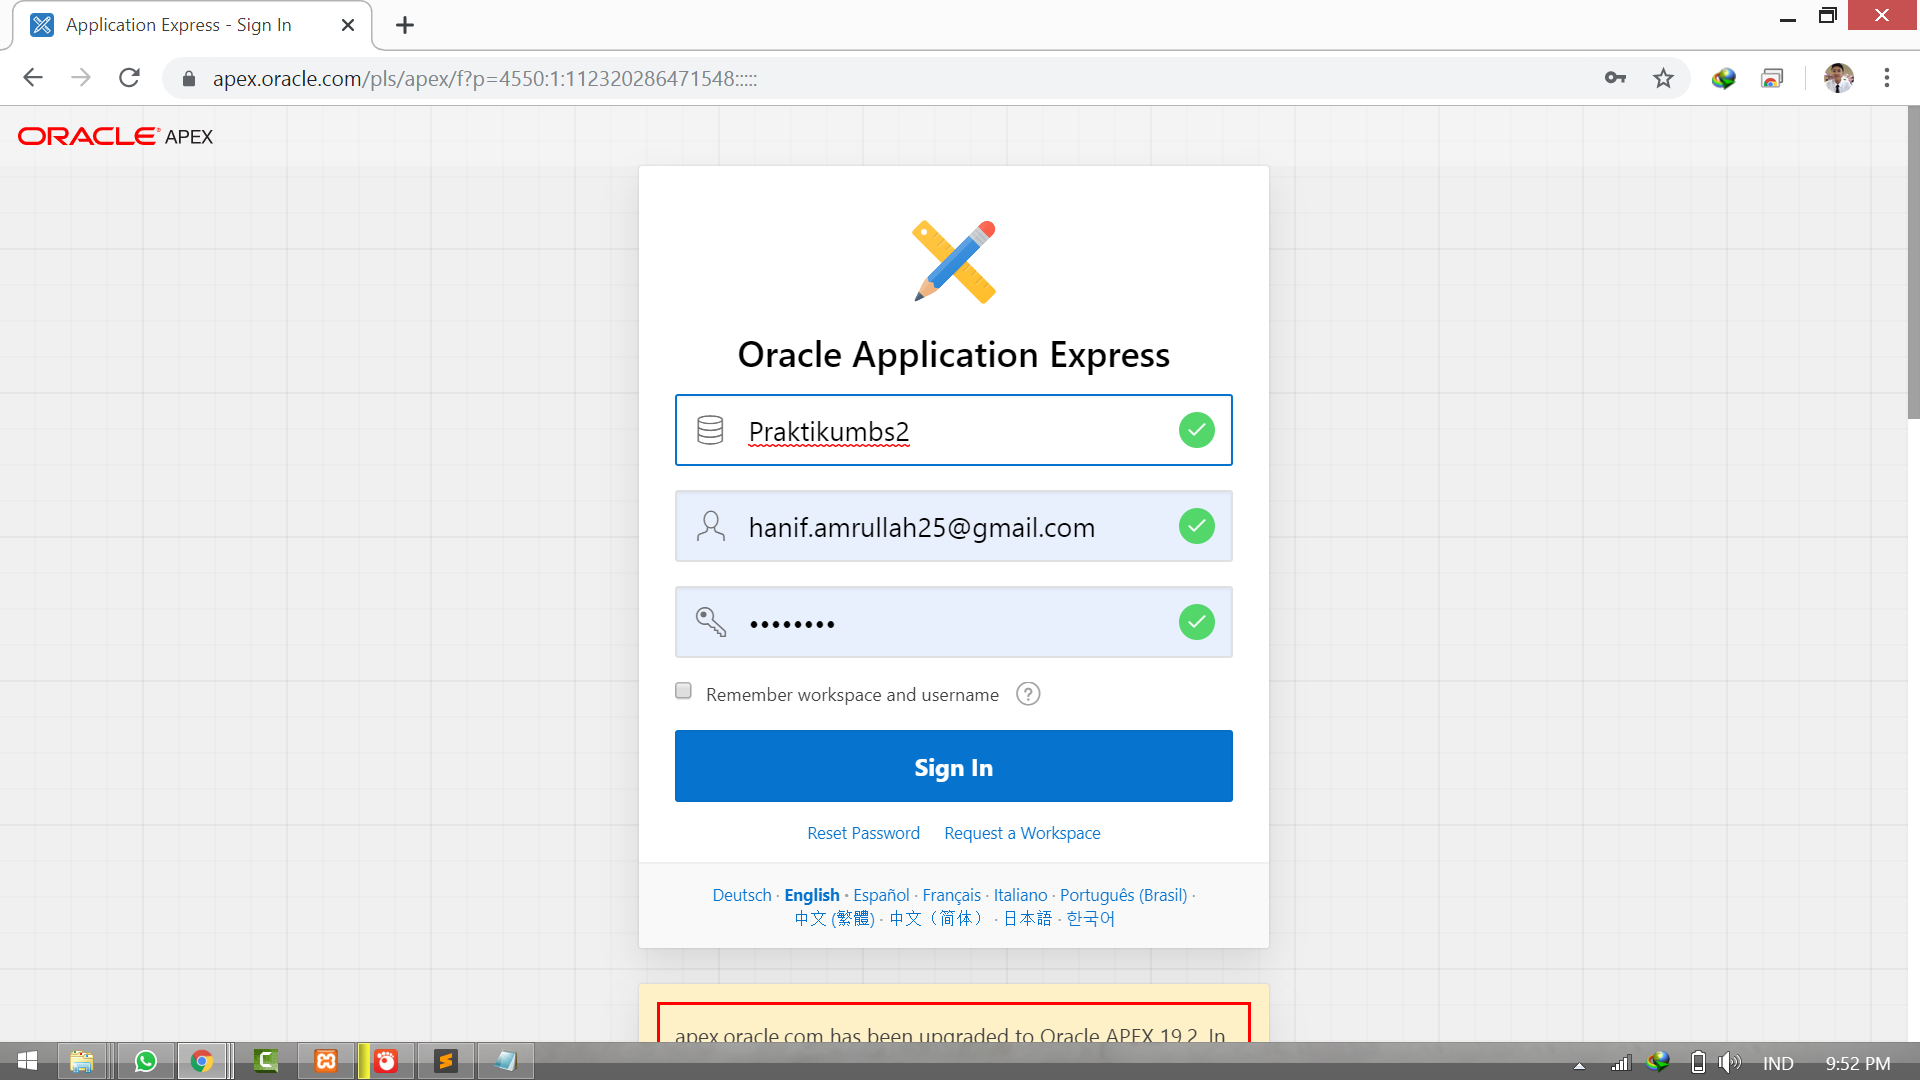
\includegraphics[width=8cm]{figure/1.png}}
\end{figure}
\begin{figure}[h]
\centerline{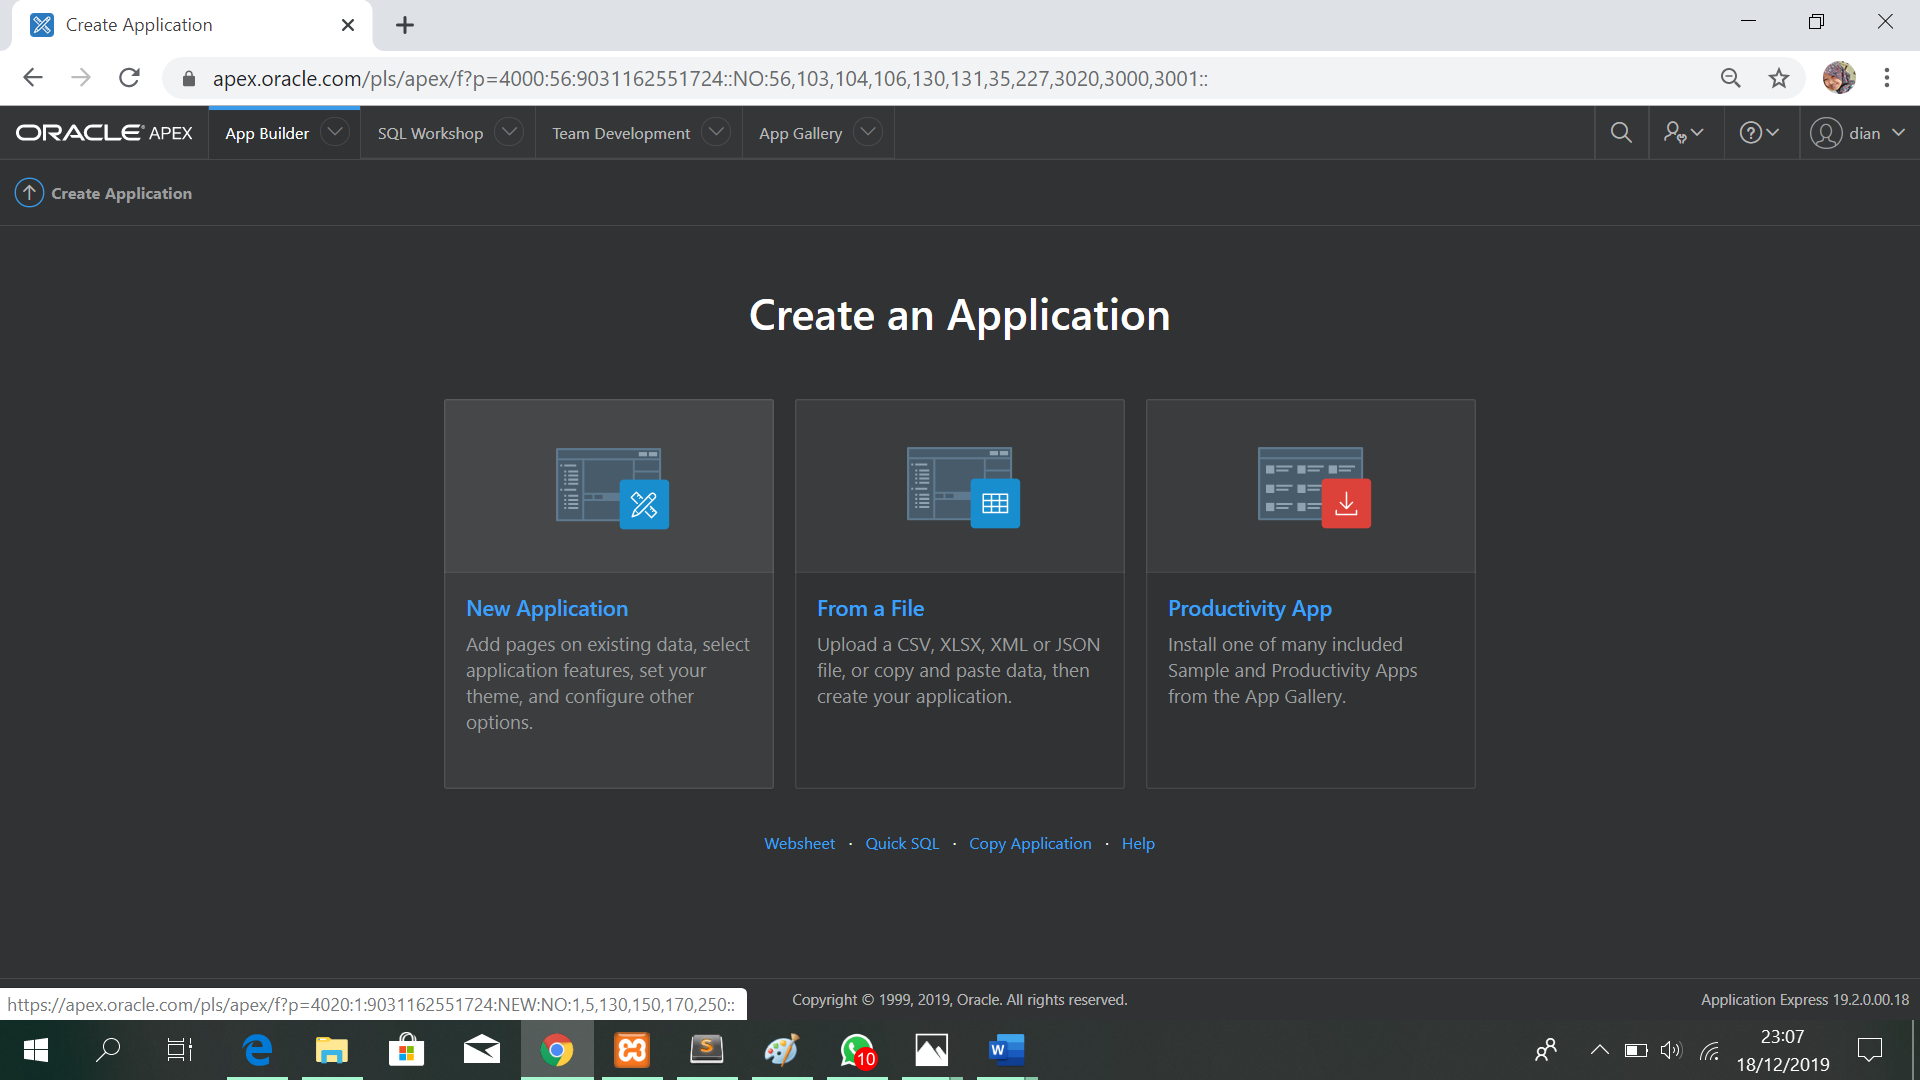
\includegraphics[width=8cm]{figure/2.png}}
\end{figure}
\begin{figure}[h]
\centerline{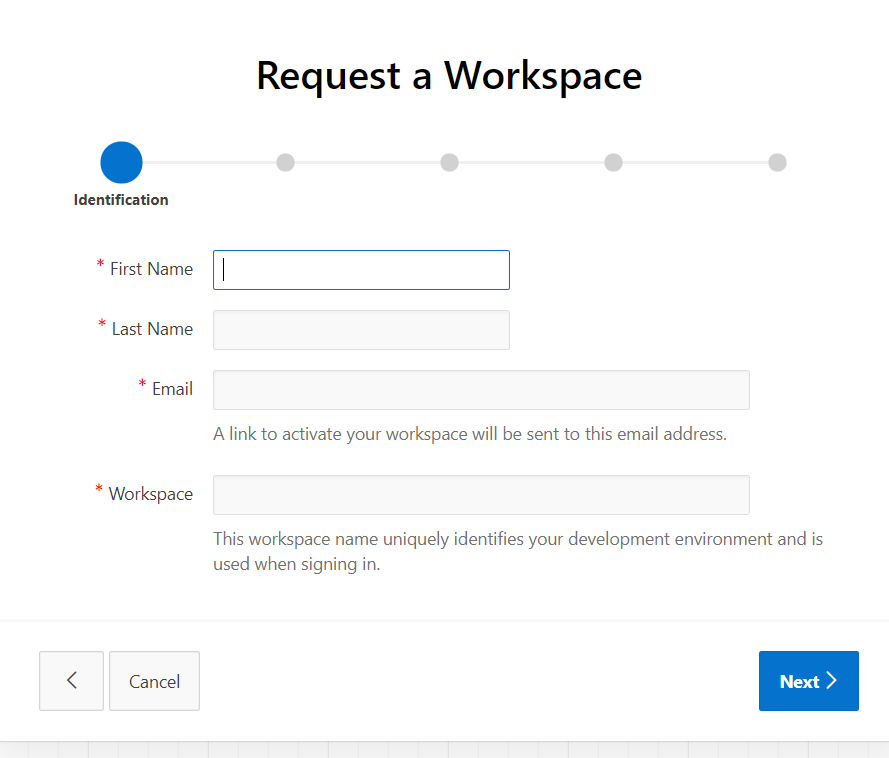
\includegraphics[width=8cm]{figure/3.png}}
\end{figure}
\begin{figure}[h]
\centerline{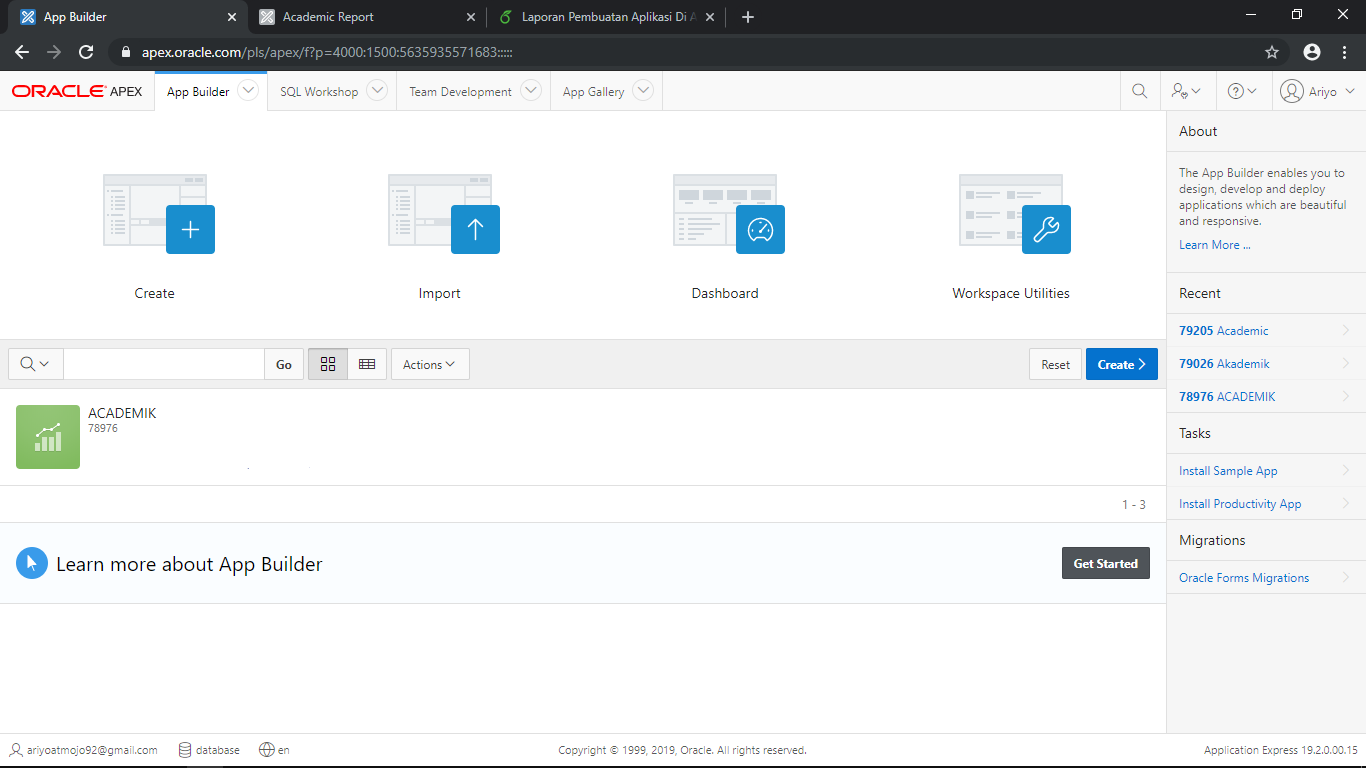
\includegraphics[width=8cm]{figure/4.png}}
\end{figure}
\newpage \begin{figure}[h]
\centerline{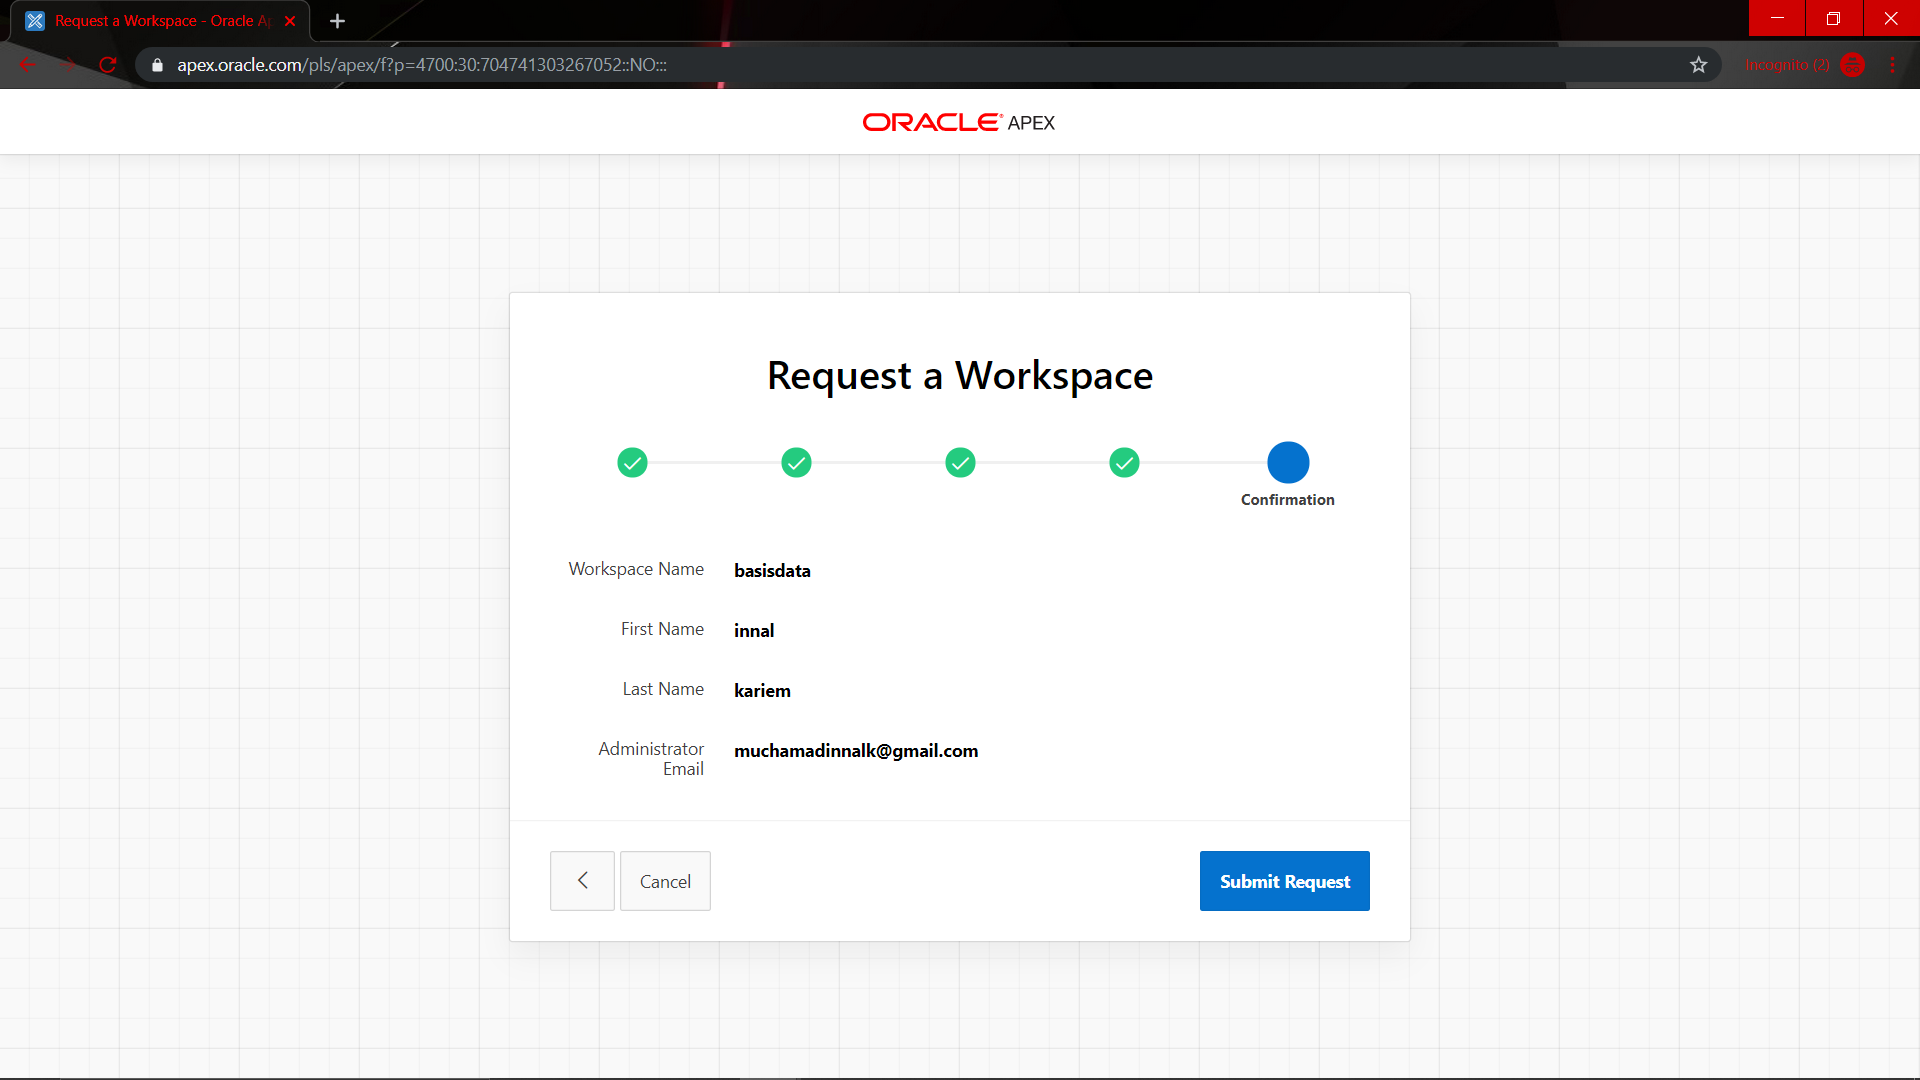
\includegraphics[width=8cm]{figure/5.png}}
\end{figure}

\newpage \par Catatan perhatikan data yang ada pada excel karena ketika ada kesalahan dalam pembuatan data contohnya baris yang kosong tetapi masuk ke dalam data maka akan mempengaruhi data pada saat mencreate aplikasi. Dan jangan lupa untuk mernomalisasi data yang telah ada. 
\item Buka aplikasi Oracle Apex terlebih dahulu
 \begin{figure}[h]	
 \centerline{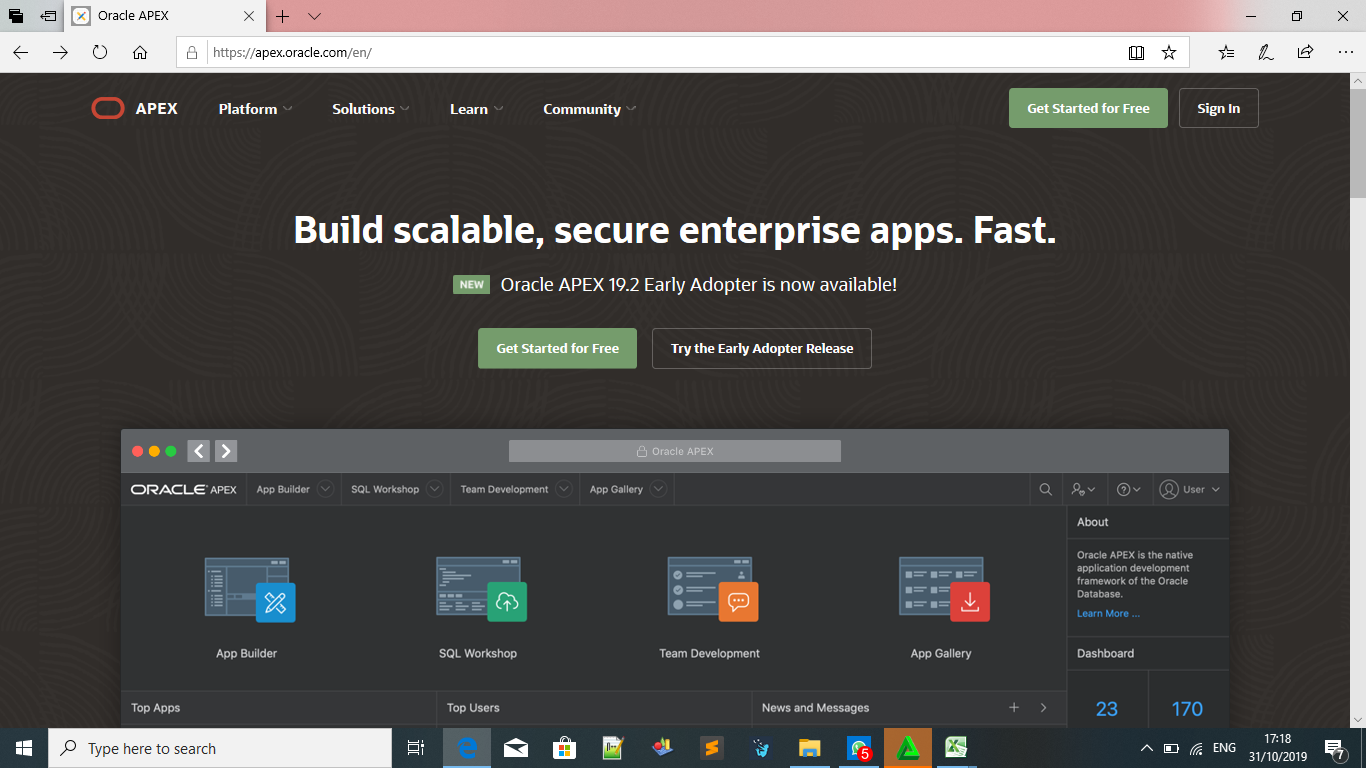
\includegraphics[width=8cm]{figure/sa.png}}
    \end{figure}
     \item Setelah itu masukkan workspace,username,dan password
         \begin{figure}[h]
    \centerline{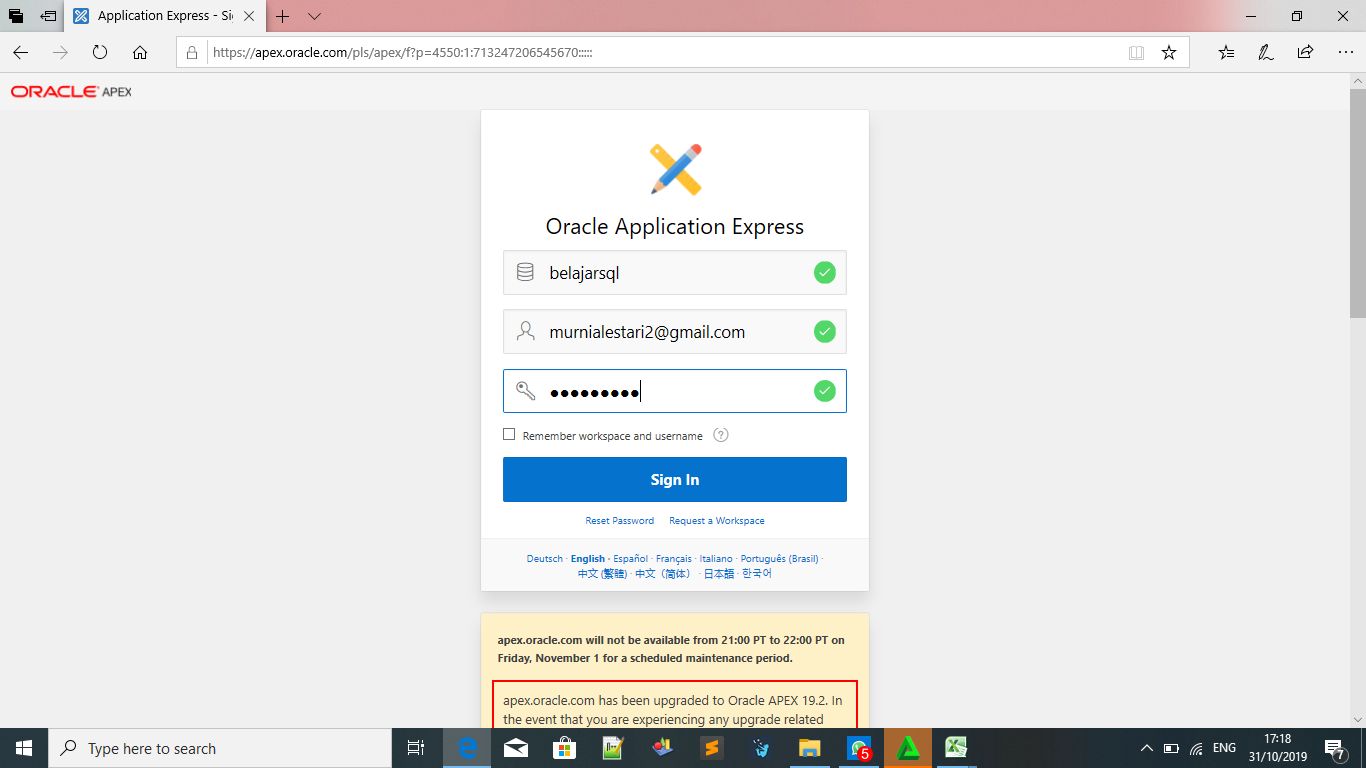
\includegraphics[width=8cm]{figure/su.png}}
       \end{figure}
\newpage \item Setelah itu pilih App builder
    \begin{figure}[h]
    \centerline{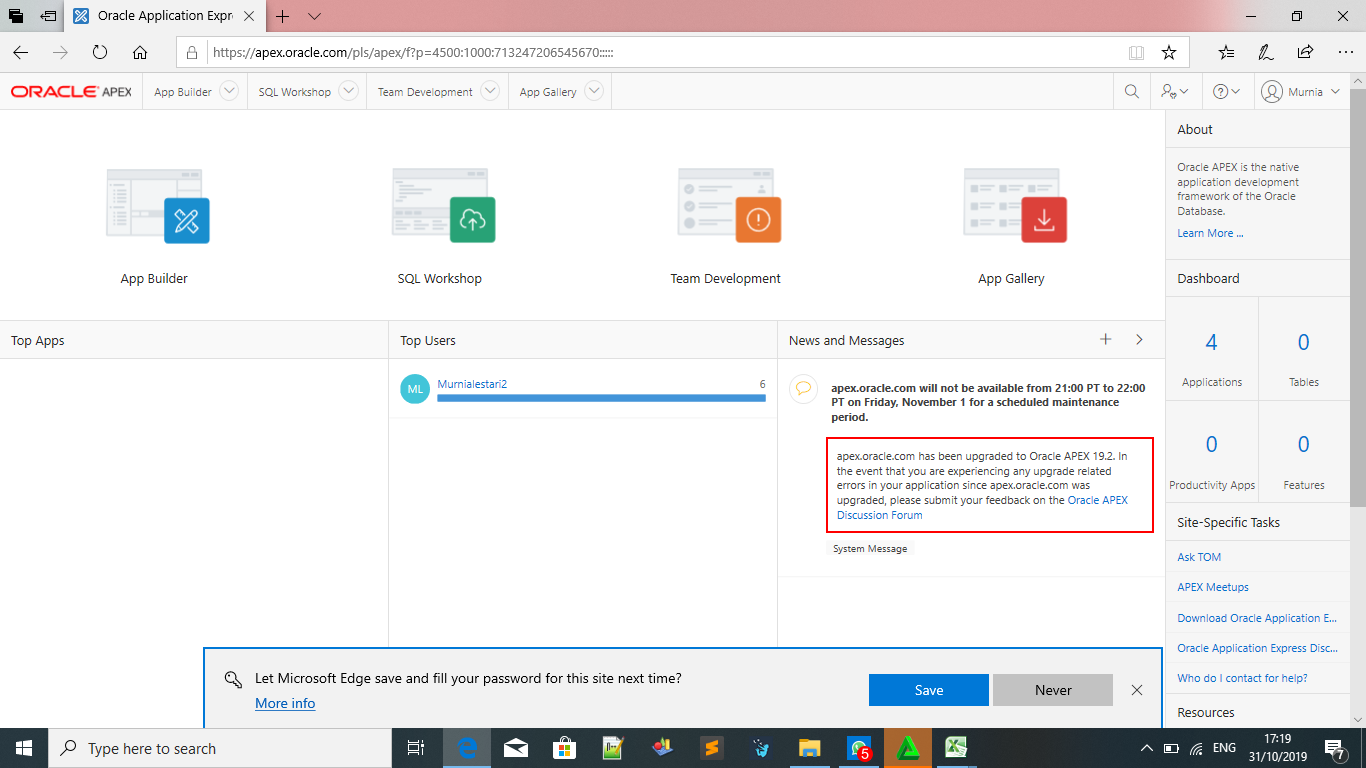
\includegraphics[width=8cm]{figure/bi.png}}
\end{figure}
  \item Setelah itu pilih create
    \begin{figure}[h]
  \centerline{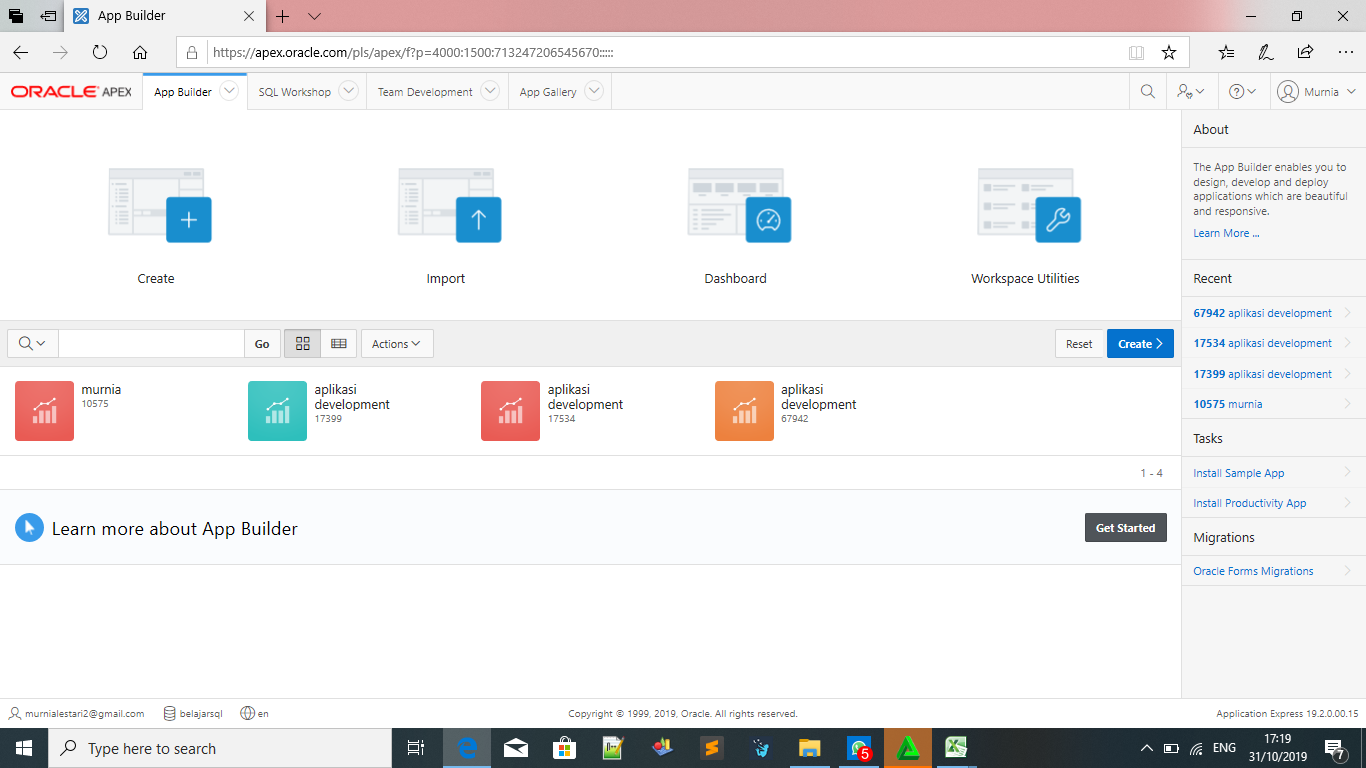
\includegraphics[width=8cm]{figure/la.png}}
\end{figure}
     \item Setelah itu pilih form a file
    \begin{figure}[h]
   \centerline{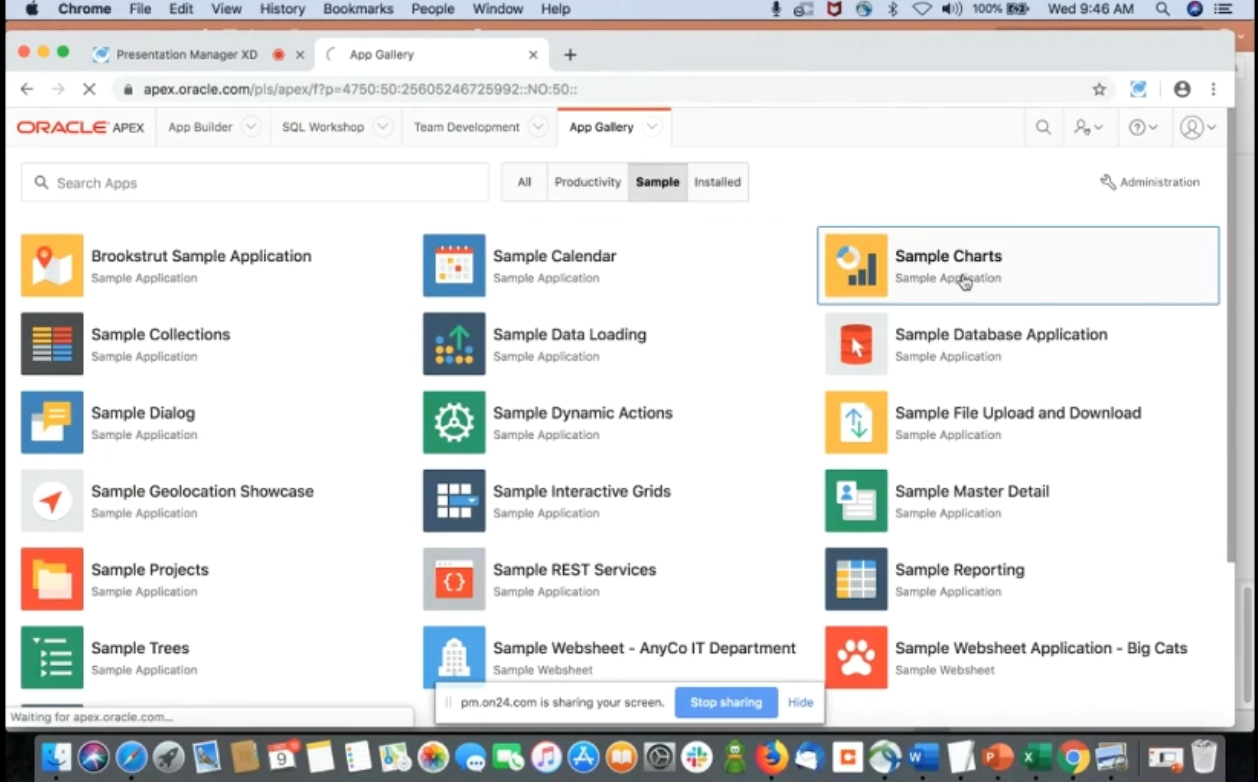
\includegraphics[width=8cm]{figure/c.PNG}}
   \end{figure}
\newpage\item lalu pilih file yang ingin kalian masukkan
    \begin{figure}[h]
   \centerline{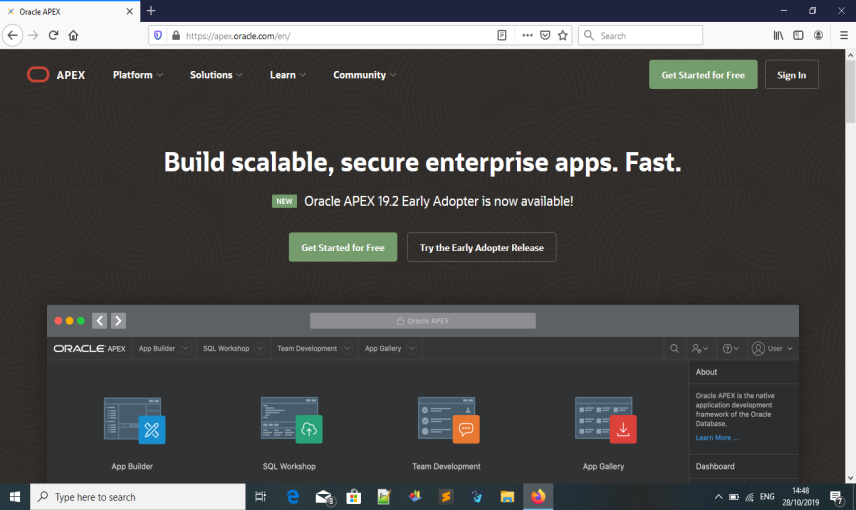
\includegraphics[width=8cm]{figure/si.png}}
\end{figure}
\item Masukkan file excel yang telah dibuat tadi
\begin{figure}[h]
   \centerline{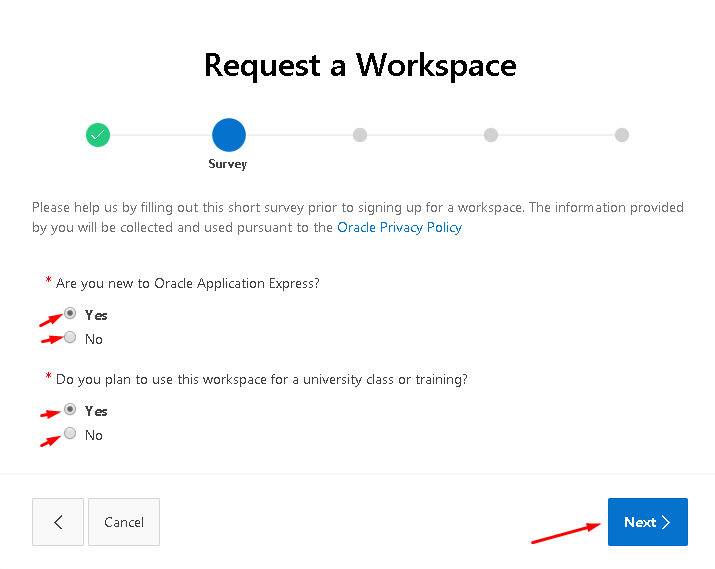
\includegraphics[width=8cm]{figure/d.png}}
\end{figure}
\newpage \item Setelah file dimasukkan isi nama table yang kamu mau contohnya  Mahasiswa
\begin{figure}[h]
\centerline{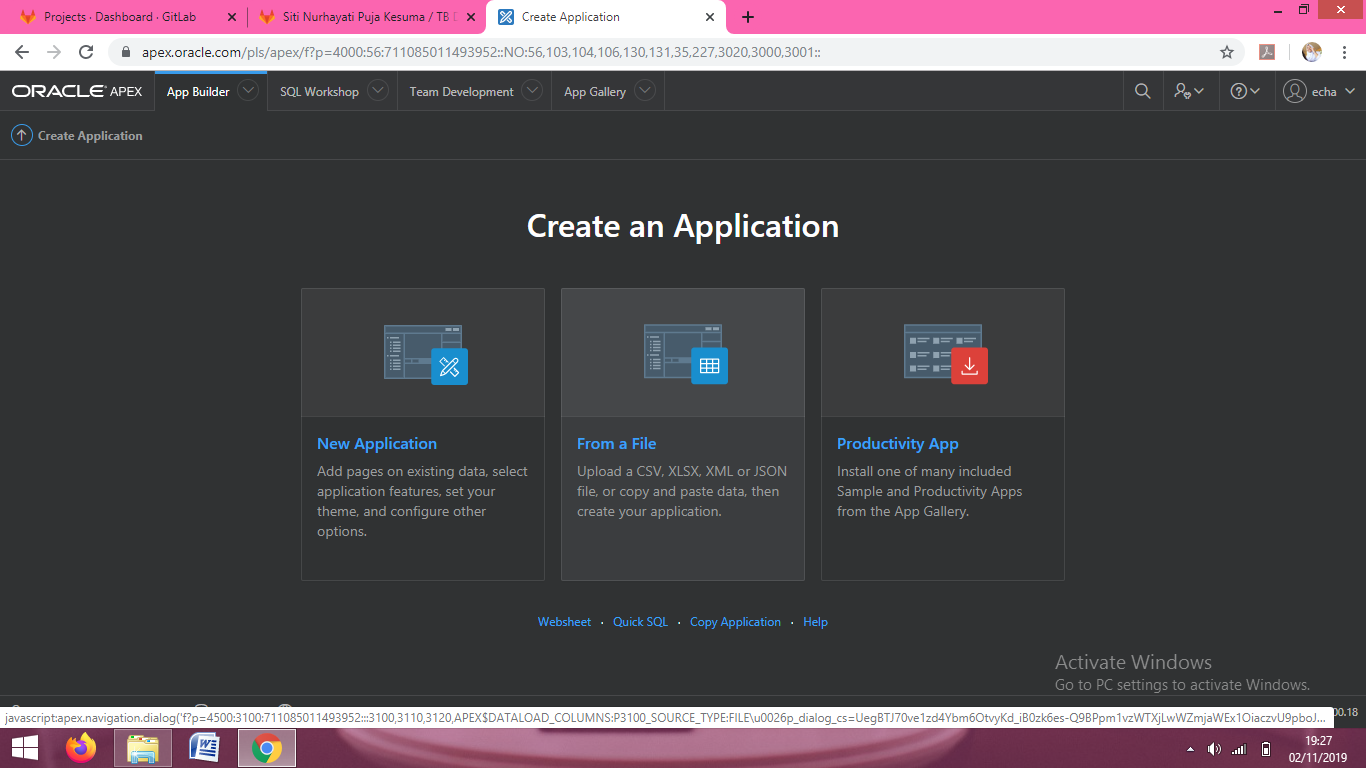
\includegraphics[width=8cm]{figure/e.png}}
\end{figure}
\item Lalu pada selectsheet jangan lupa pilih mahasiswa karena pada file excel terdapat sheet yang berbeda-beda namanya yaitu Mahasiswa,Dosen,Mata Kuliah,Nilai,dan Jadwal. Pilih Mahasiswa untuk mengupload excel yang pertama.
\begin{figure}[h]
\centerline{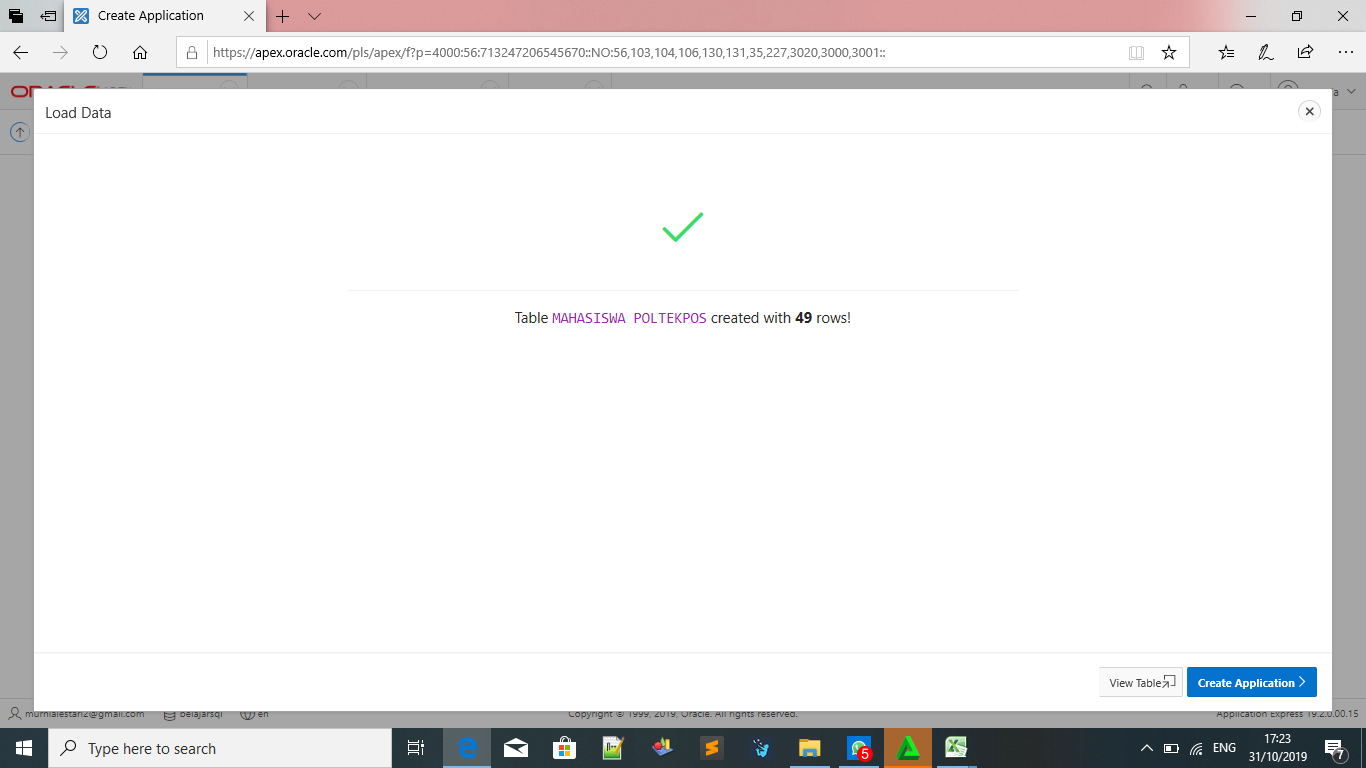
\includegraphics[width=8cm]{figure/di.png}}
\end{figure}
\newpage \item Untuk memastikan apakah file yang dimasukkan telah masuk maka pilih configure. Terkadang di dalam file yang kita masukkan terdapat tabel yang kosong maka hapus ceklis yang pada kolom tersebut karena akan mempengaruhi ketika pembuatan aplikasi.
\begin{figure}
\centerline{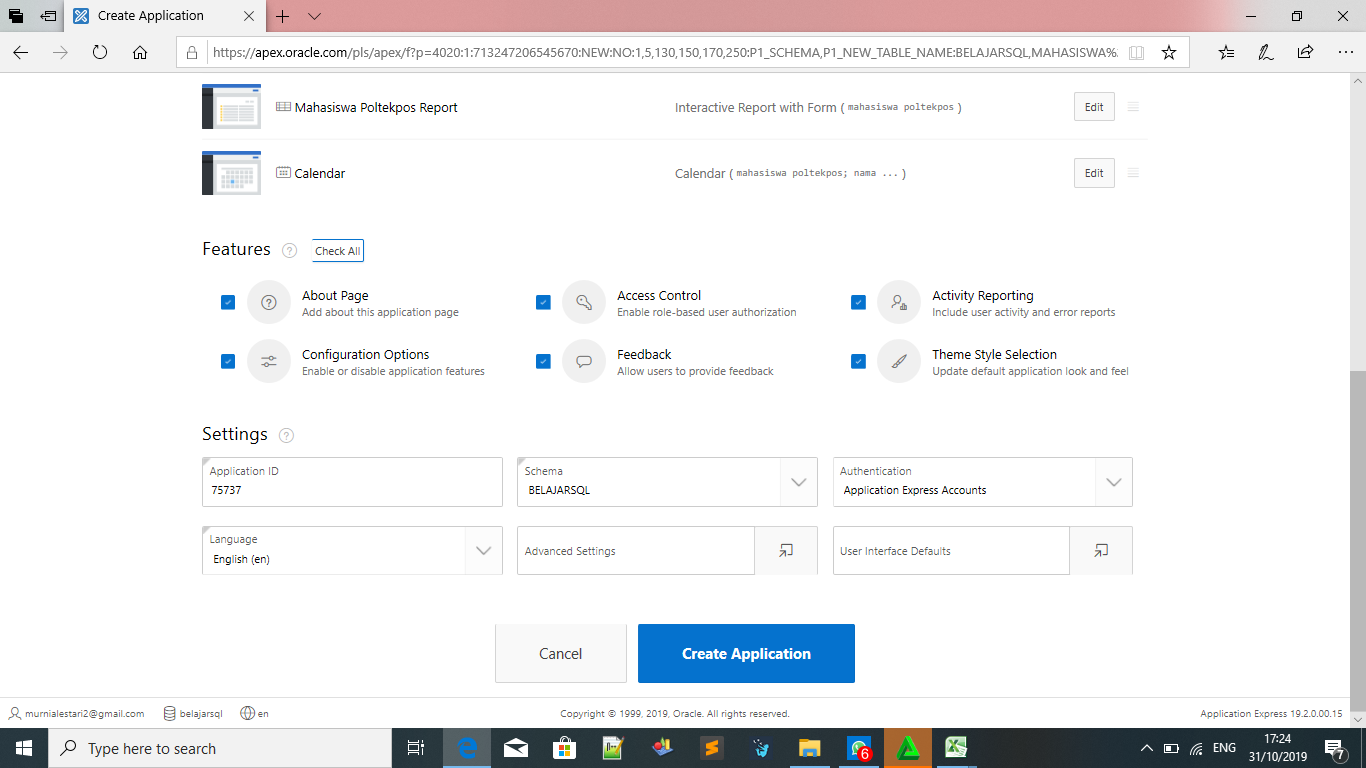
\includegraphics[width=8cm]{figure/da.png}}
\end{figure}
\item Lalu pilih Save Change
\item Lalu pilih load data dan finish
 \item Lakukan hal yang sama untuk data yang lain, lanjutkan ke selectsheet pilih Dosen. Lalu pilih configure, kemudian lihat file yang dimasukkan lalu pilih save change, load data dan finish.
\newpage \begin{figure}
\centerline{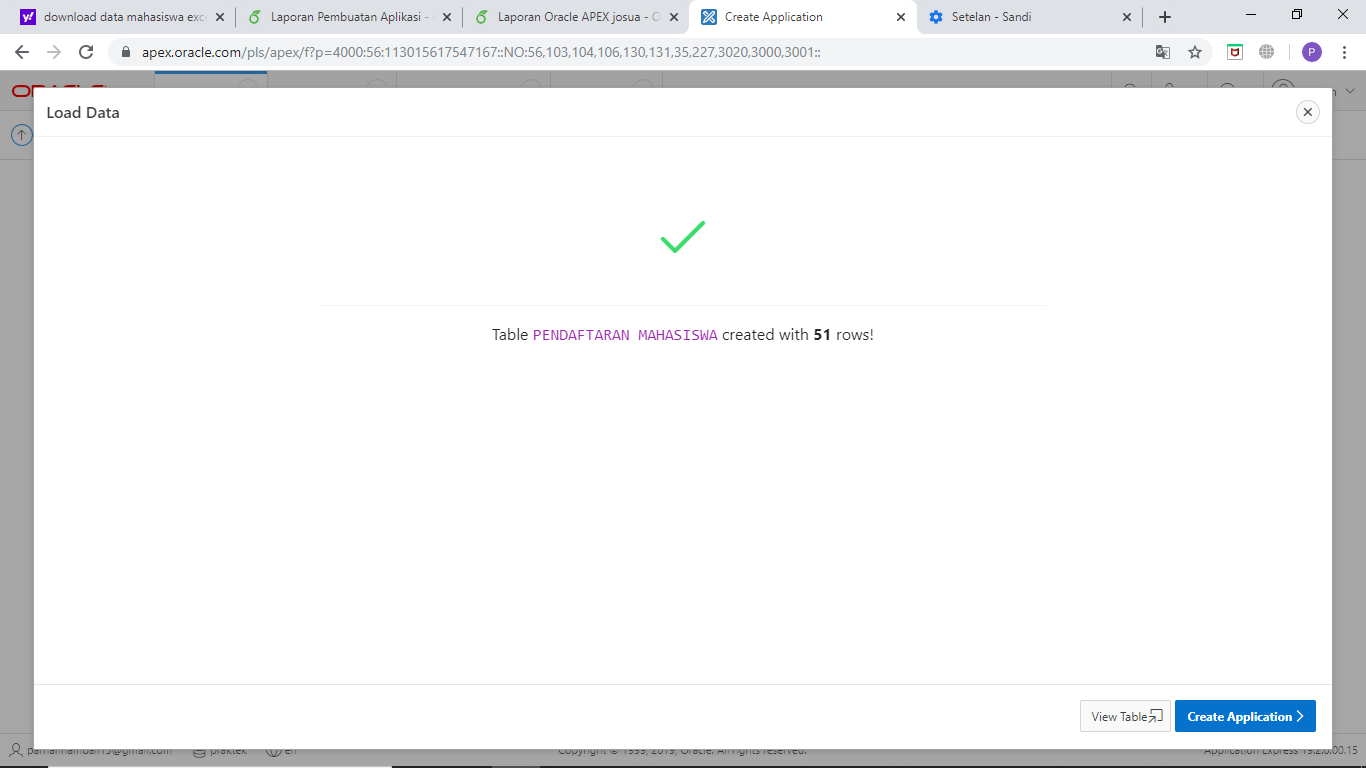
\includegraphics[width=8cm]{figure/8.png}}
\end{figure}
\begin{figure}
\centerline{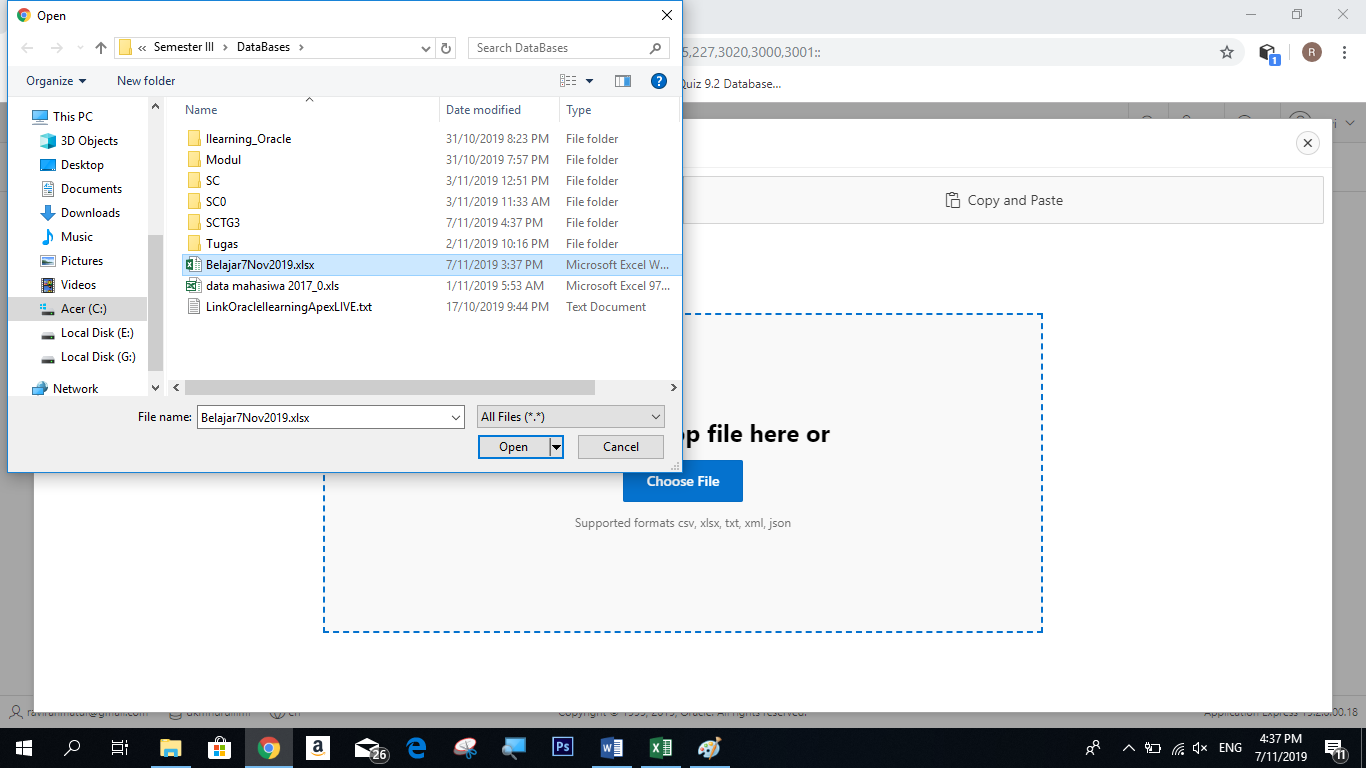
\includegraphics[width=8cm]{figure/9.png}}
\end{figure}
\begin{figure}
\centerline{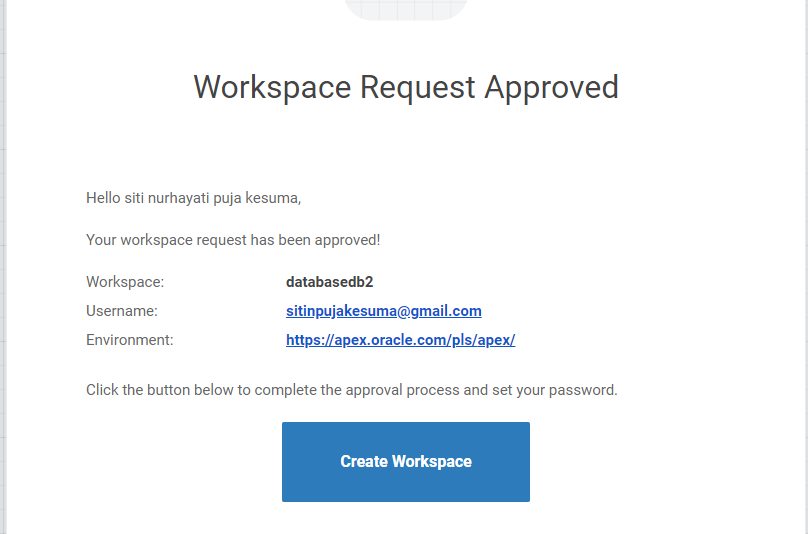
\includegraphics[width=8cm]{figure/10.png}}
\end{figure}
\newpage \item Lakukan hal yang sama untuk data yang lain, lanjutkan ke selectsheet pilih Kuliah. Lalu pilih configure, kemudian lihat file yang dimasukkan lalu pilih save change, load data dan finish.
\begin{figure}
\centerline{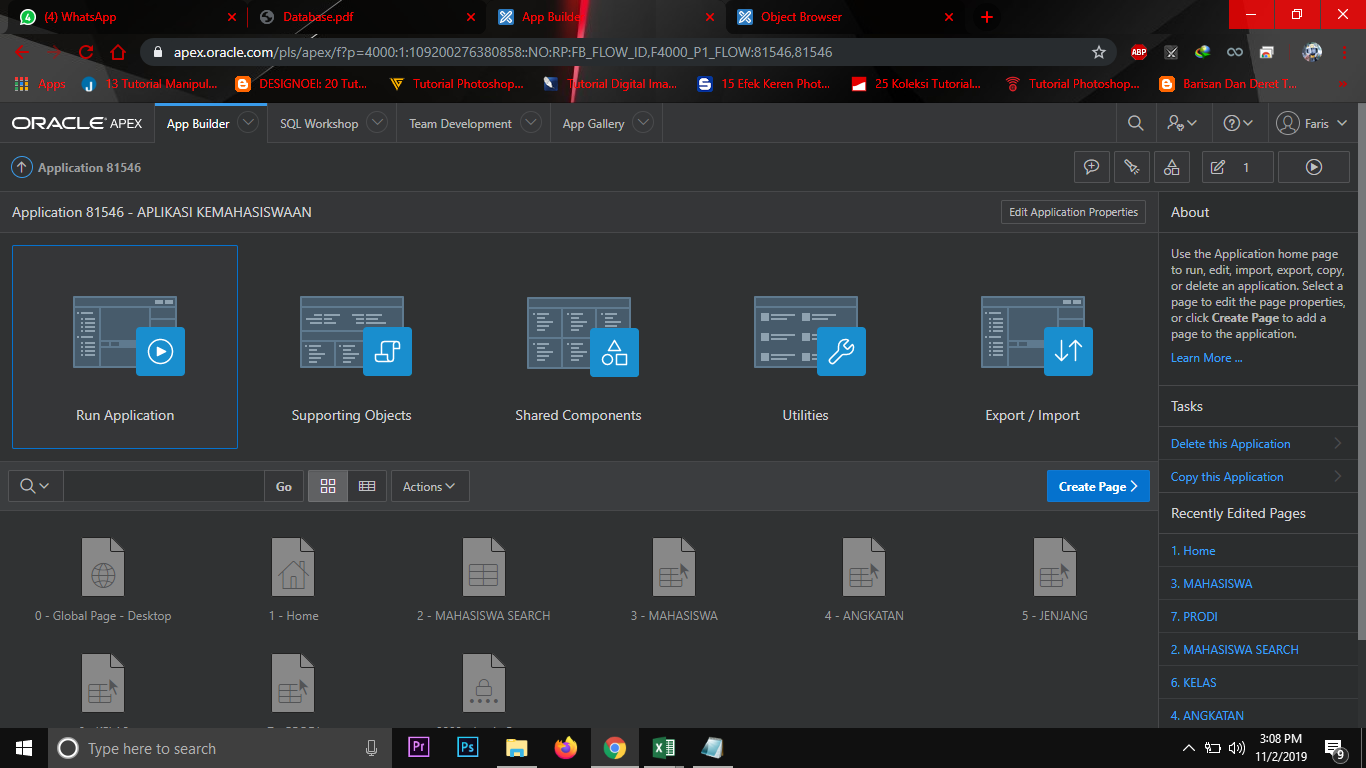
\includegraphics[width=8cm]{figure/11.png}}
\end{figure}
\begin{figure}
\centerline{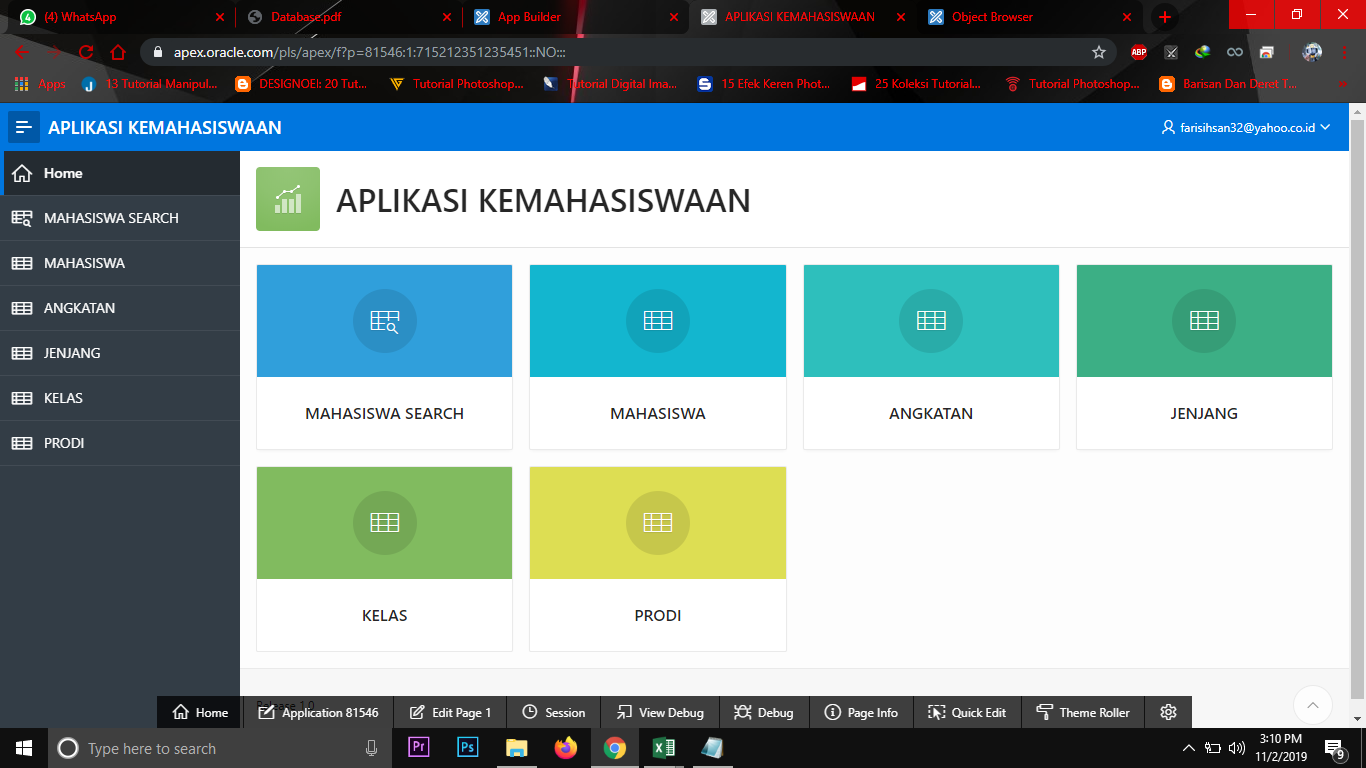
\includegraphics[width=8cm]{figure/12.png}}
\end{figure}
\begin{figure}
\centerline{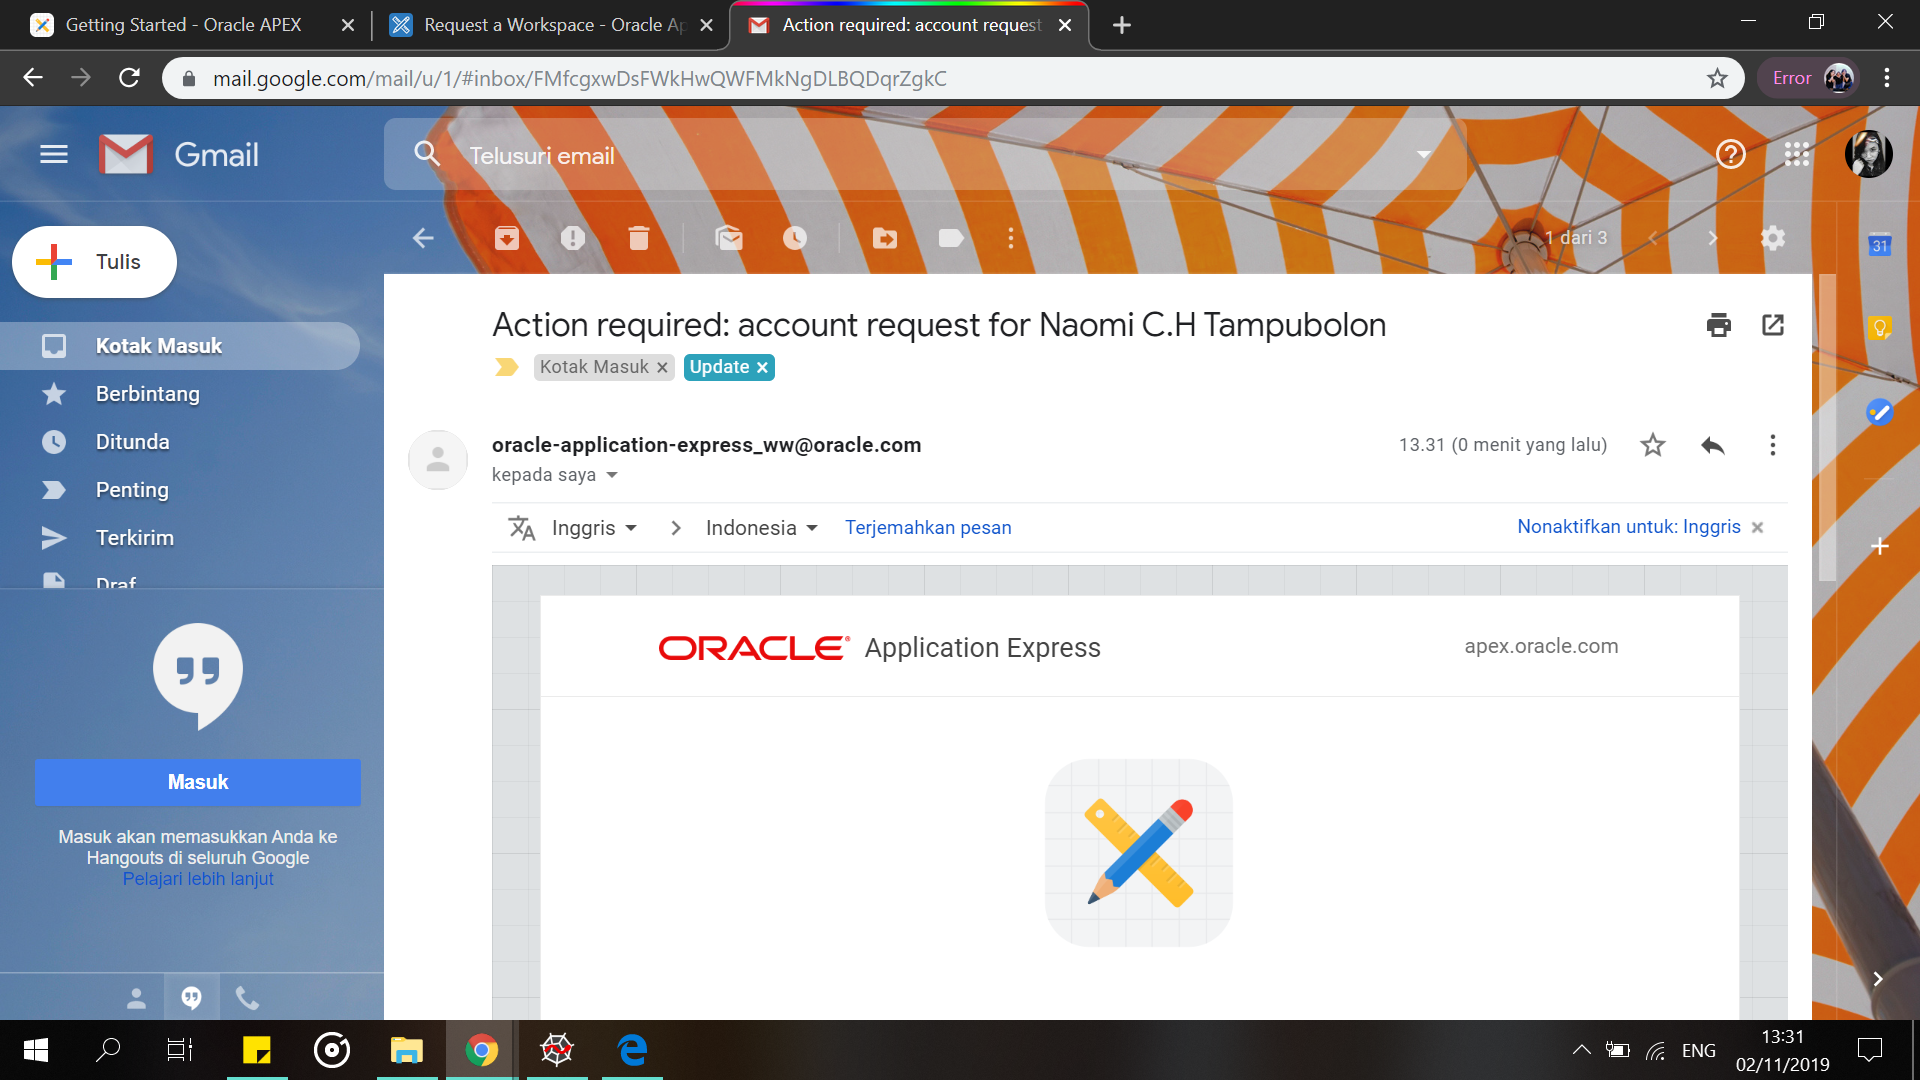
\includegraphics[width=8cm]{figure/13.png}}
\end{figure}
    
   \newpage \item Kita dapat melihat table kita pada SQL WorkShop
     \begin{center}
    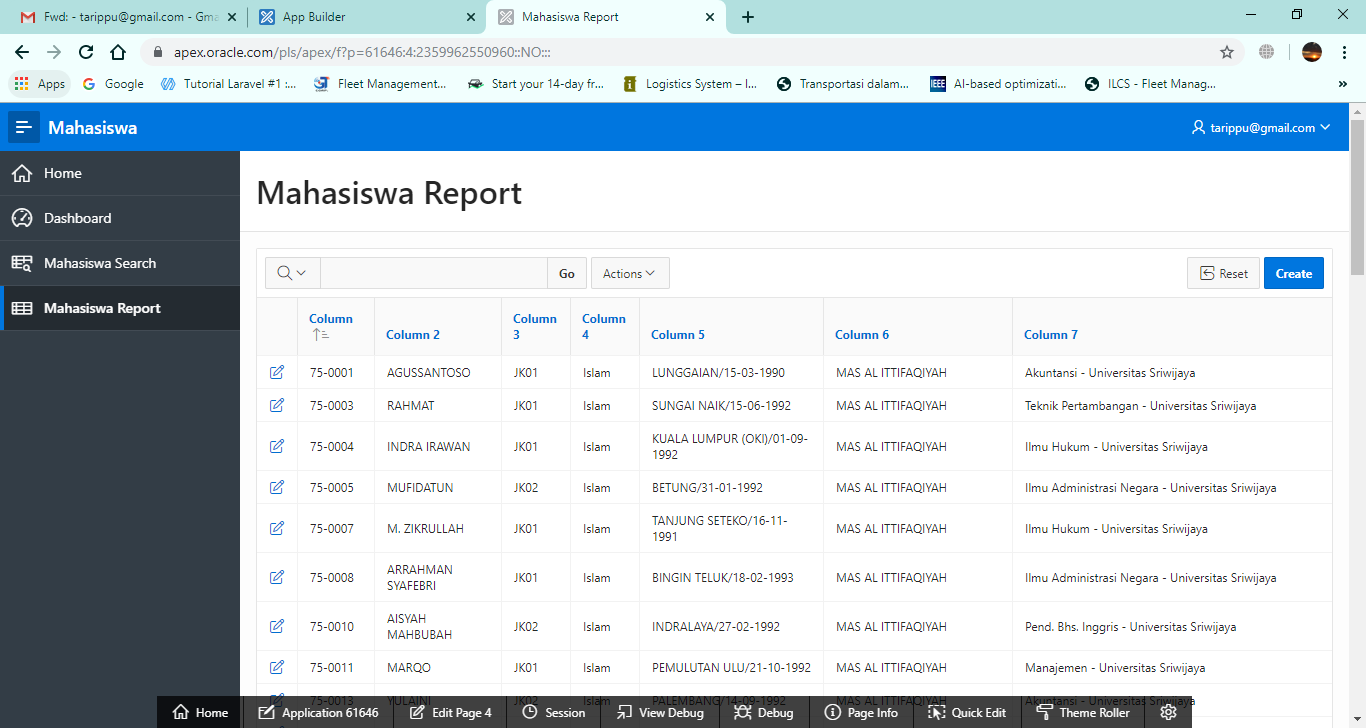
\includegraphics[width=.8\textwidth]{figure/16.PNG}
    \end{center}
    \item Hilangkan kolom ID(number) pada setiap tabel karena akan mempengaruhi file yang membuat file yang kita masukkan error.
     \begin{center}
    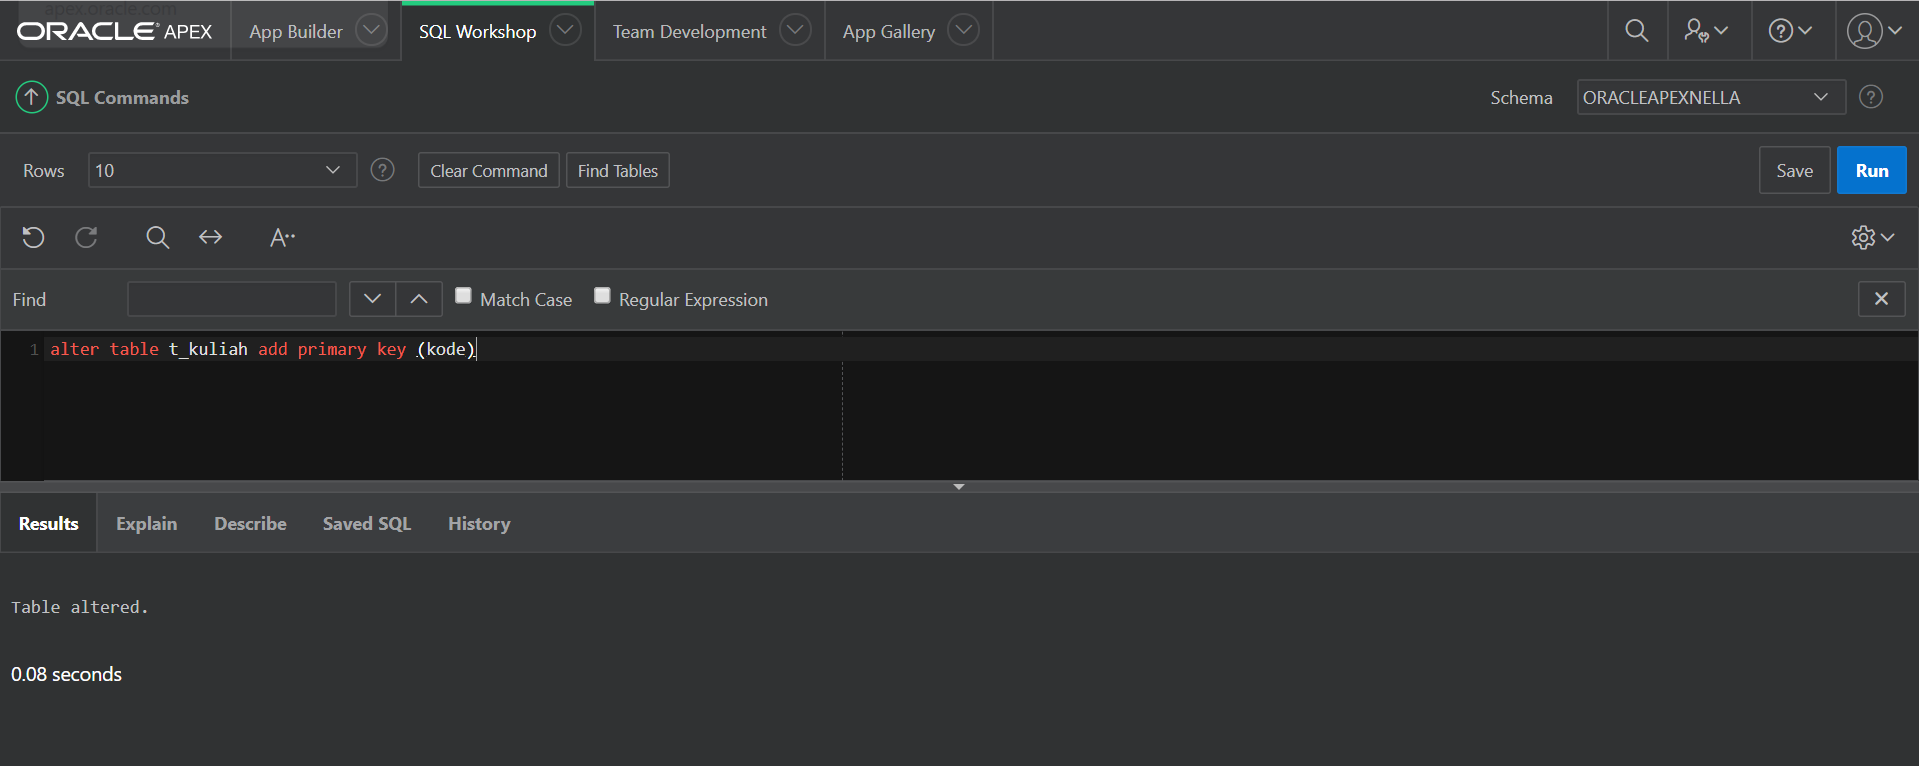
\includegraphics[width=.8\textwidth]{figure/17.PNG}
    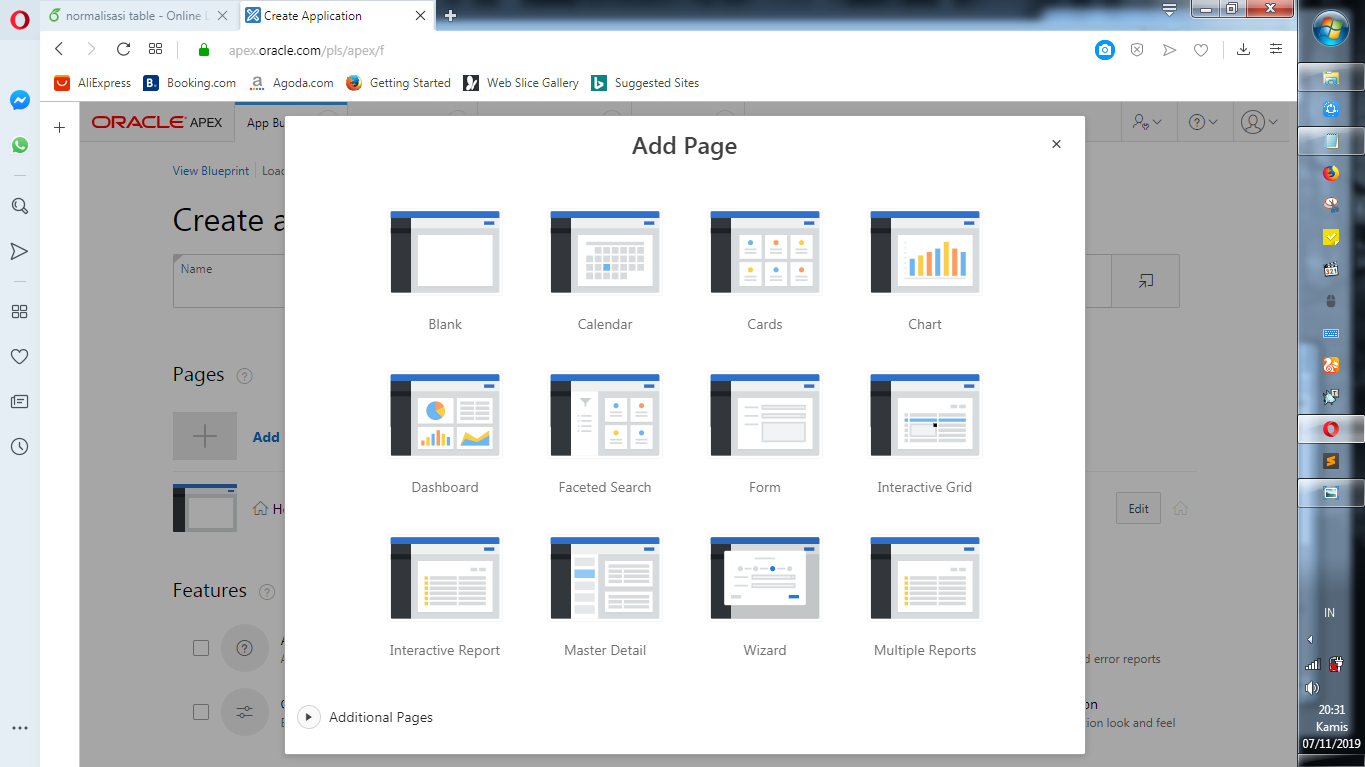
\includegraphics[width=.8\textwidth]{figure/18.PNG}
    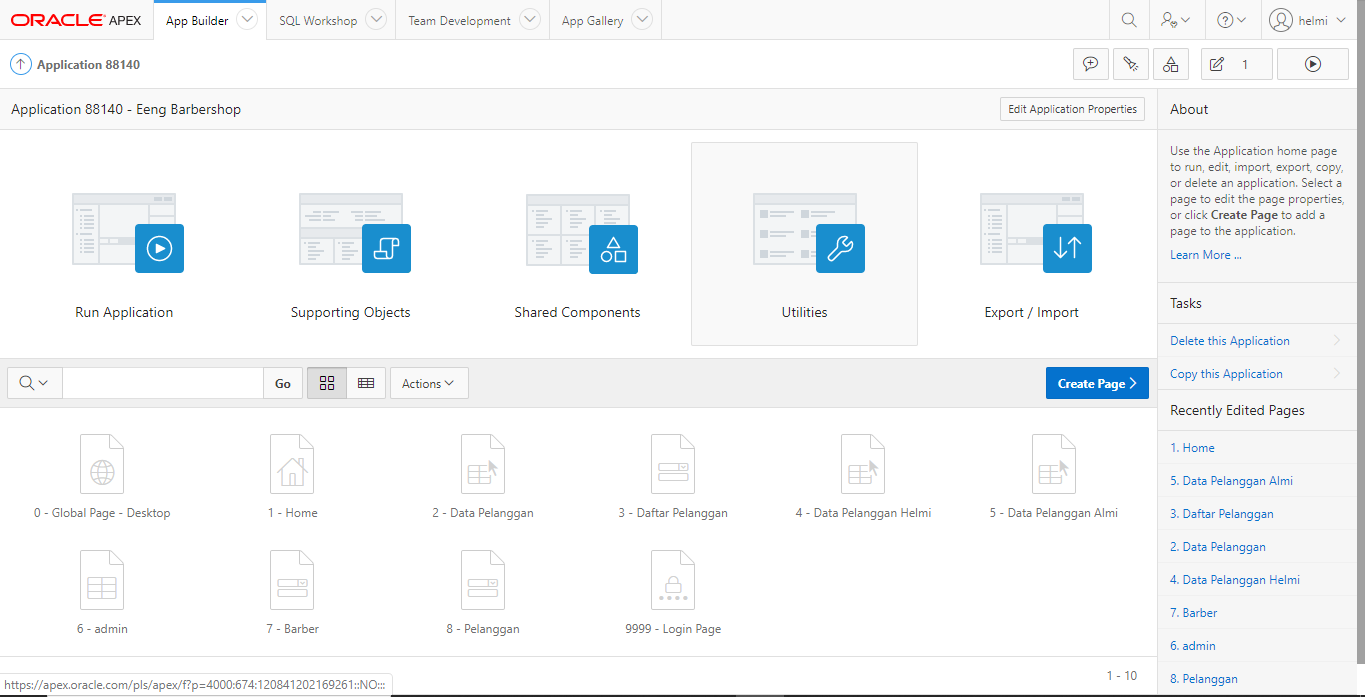
\includegraphics[width=.8\textwidth]{figure/19.PNG}
    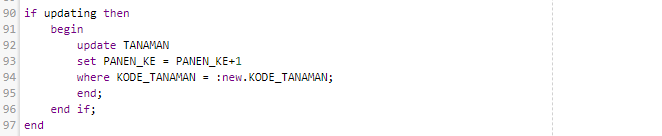
\includegraphics[width=.8\textwidth]{figure/20.PNG}
    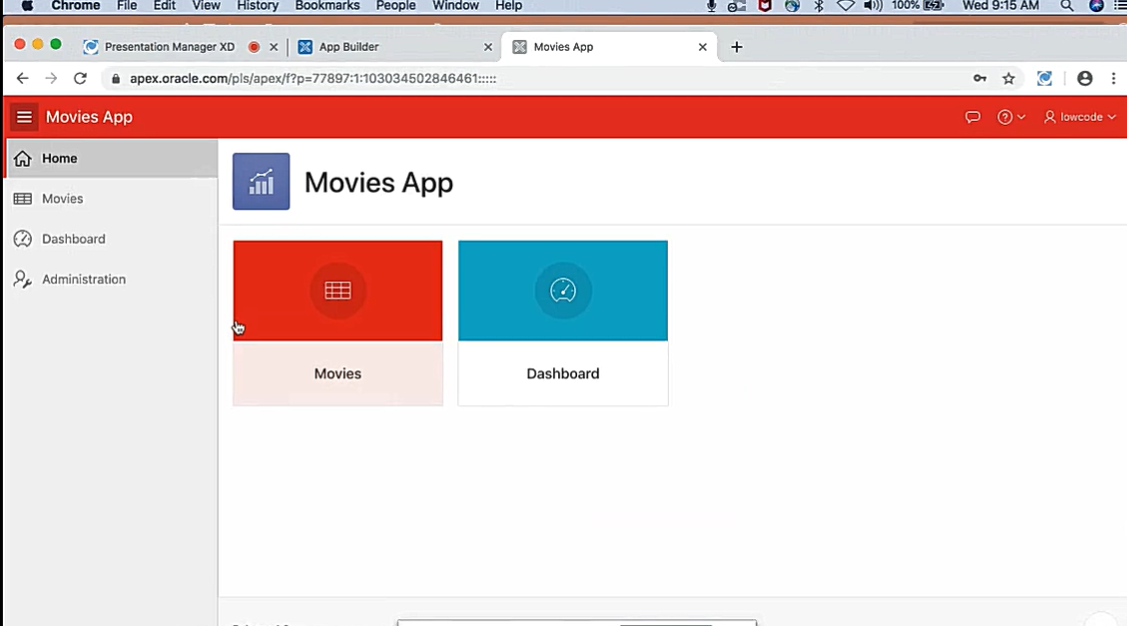
\includegraphics[width=.8\textwidth]{figure/21.PNG}
    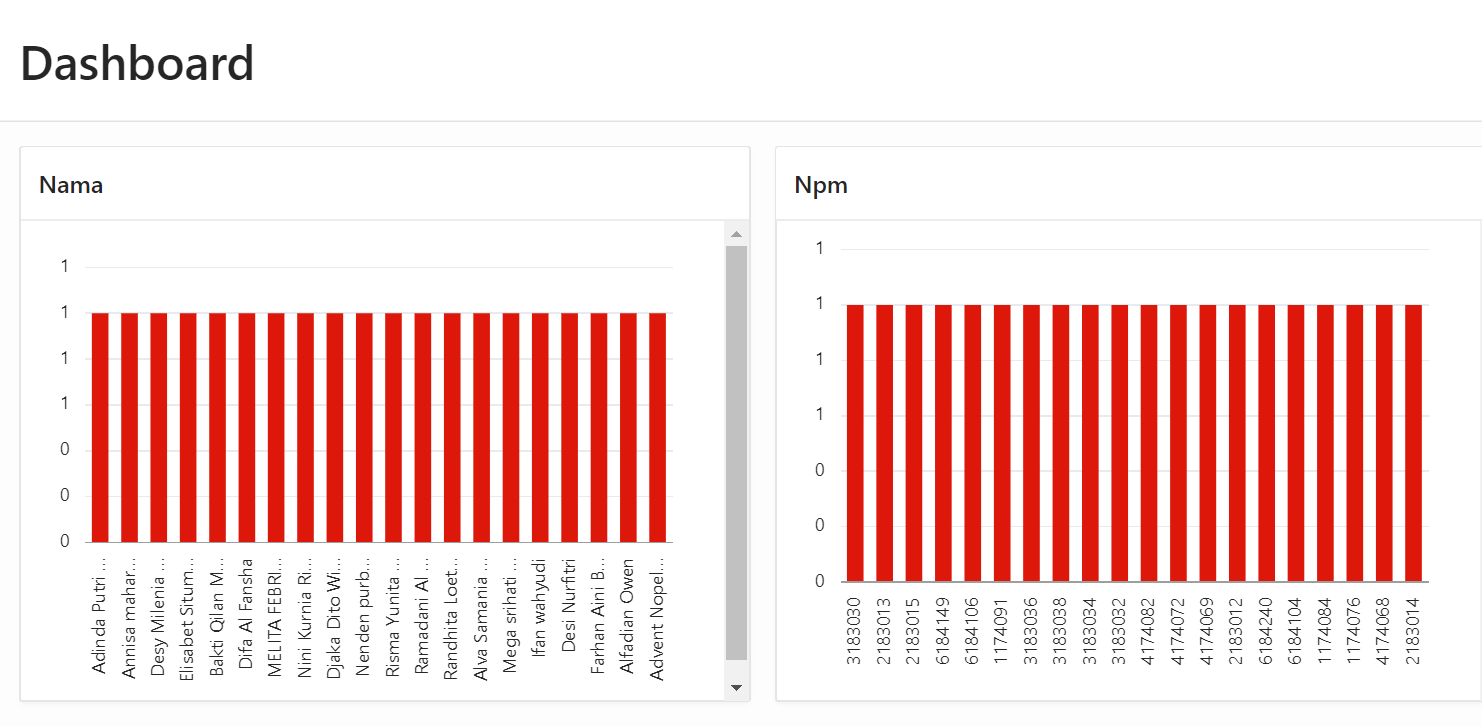
\includegraphics[width=.8\textwidth]{figure/22.PNG}
    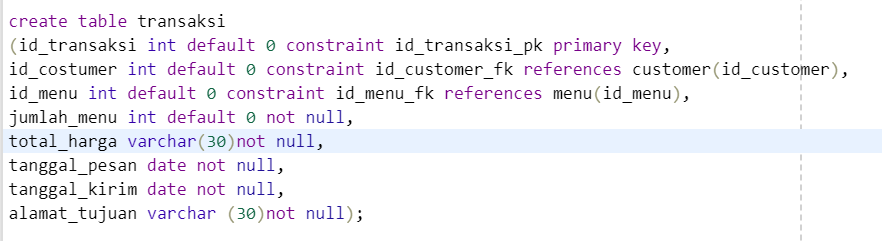
\includegraphics[width=.8\textwidth]{figure/23.PNG}
    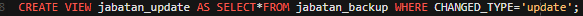
\includegraphics[width=.8\textwidth]{figure/24.PNG}
    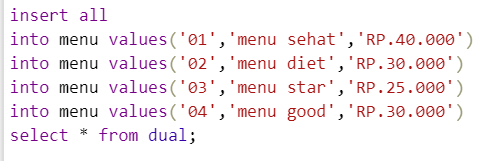
\includegraphics[width=.8\textwidth]{figure/25.PNG}
    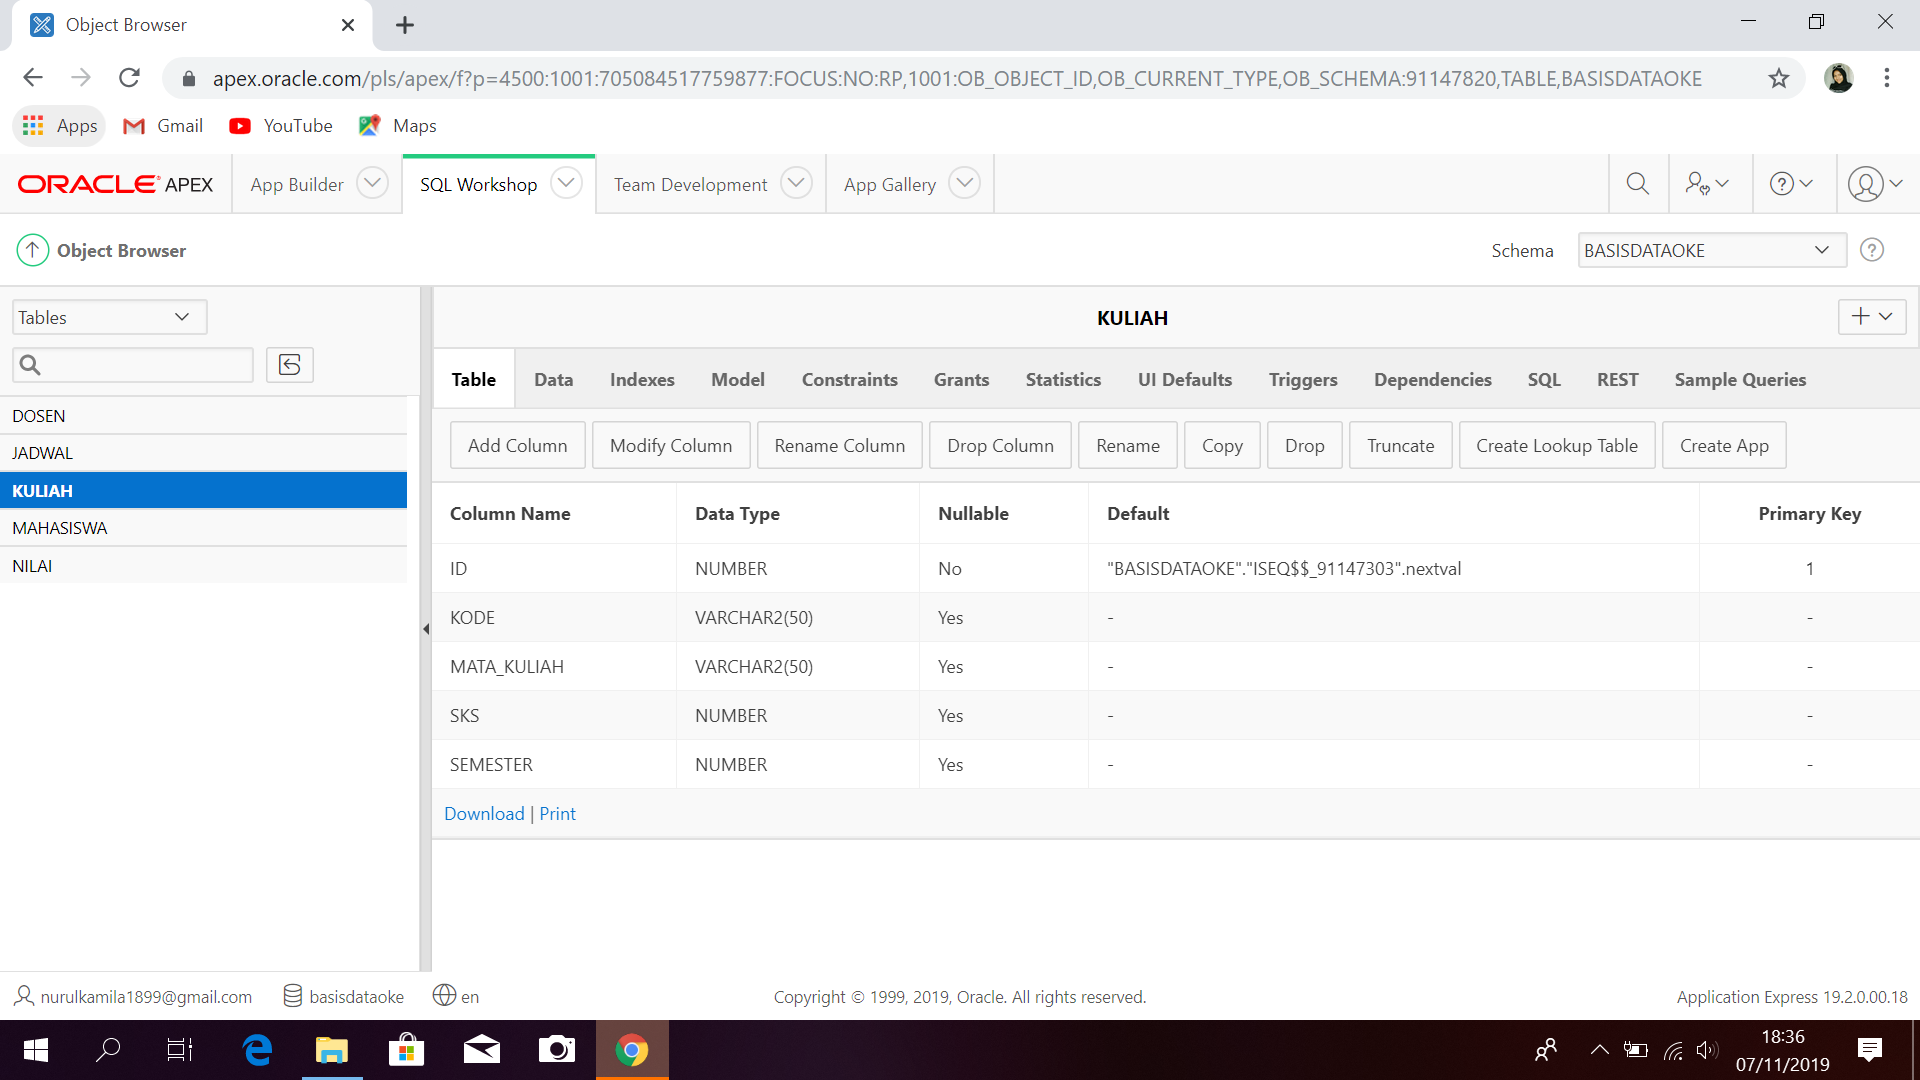
\includegraphics[width=.8\textwidth]{figure/26.PNG}
    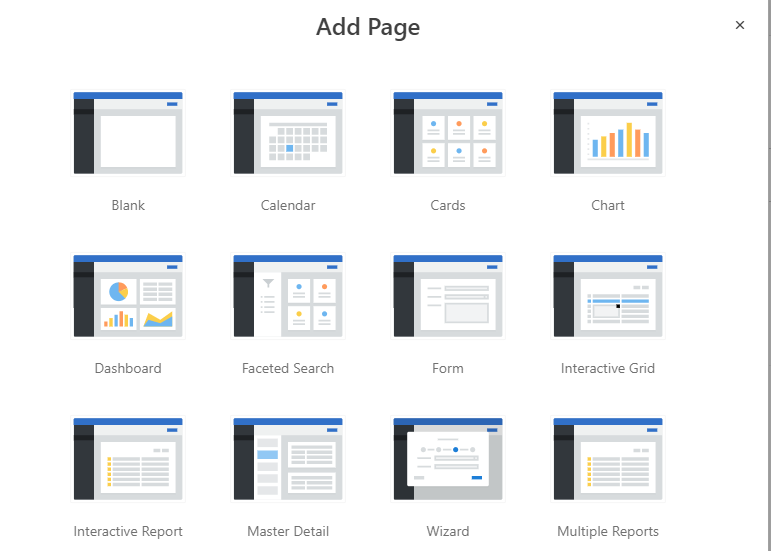
\includegraphics[width=.8\textwidth]{figure/27.PNG}
    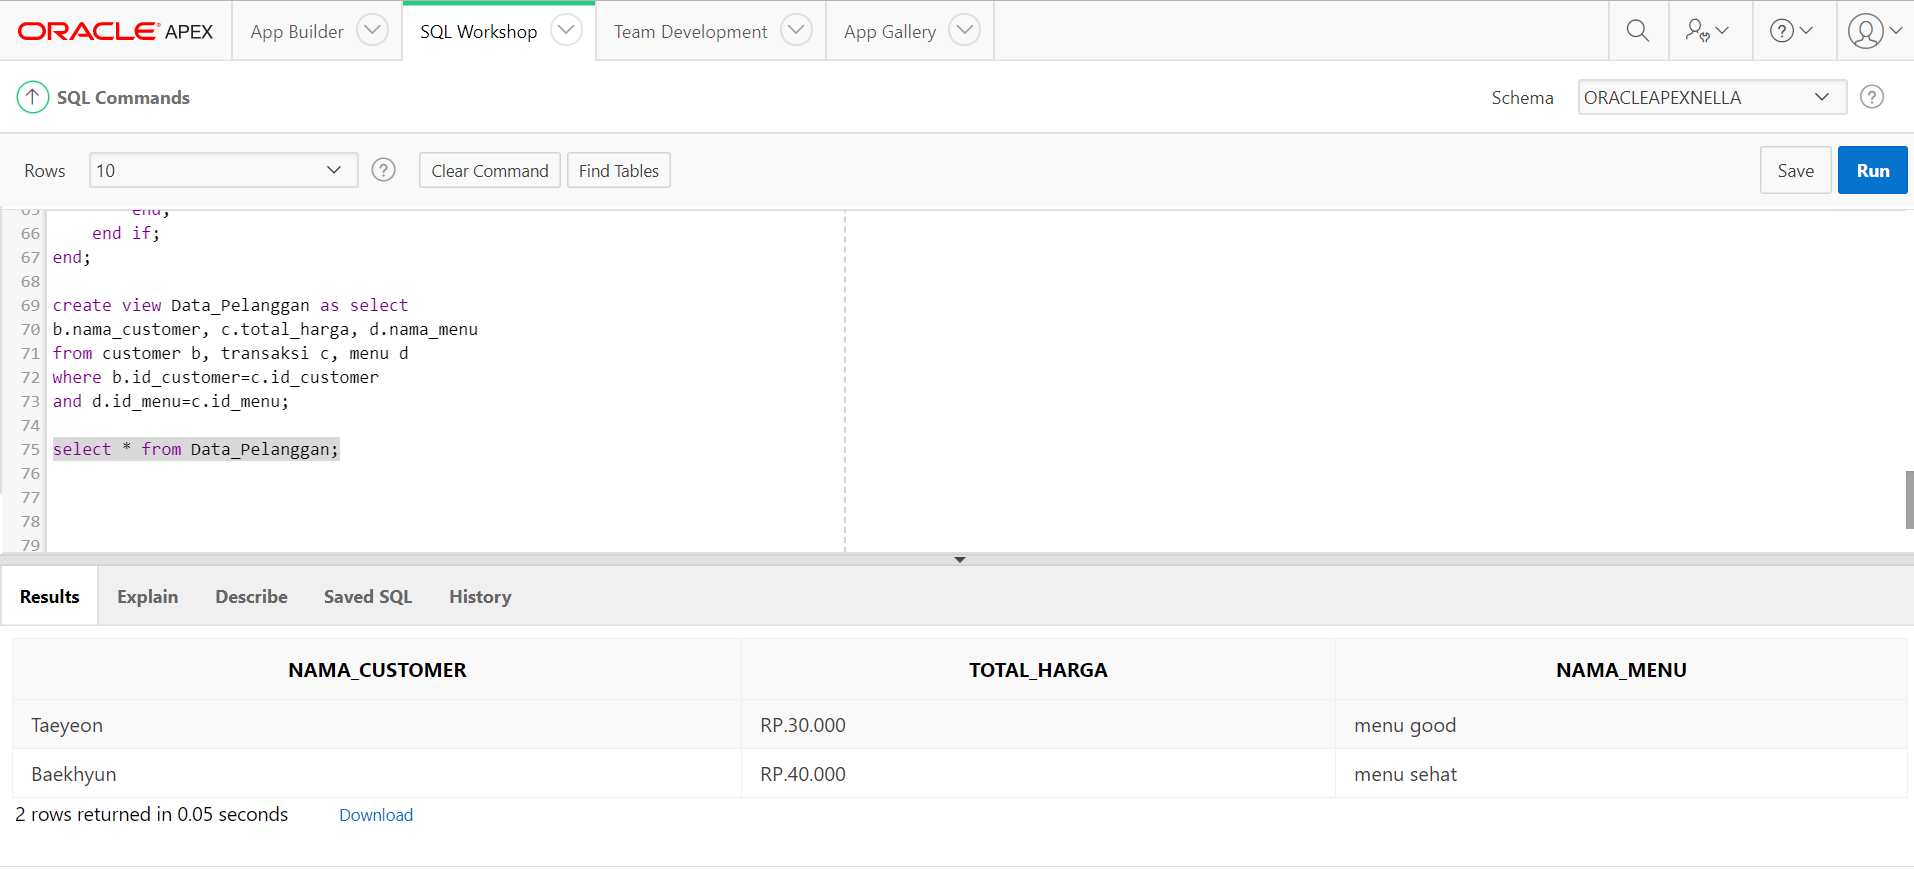
\includegraphics[width=.8\textwidth]{figure/29.PNG}
    \end{center}
    \item setelah itu, pada pilihan constrains, setting primery key pada mahasiswa yaitu NIM,pada dosen primary keynya adalah NIK,pada mata kuliah primary keynya adalah kode, dan foregent key sesuai tabel pada tabel nilai yaitu pada kode dan nim,serta jadwal foregent keynya adalah kode dan nik
    \begin{center}
    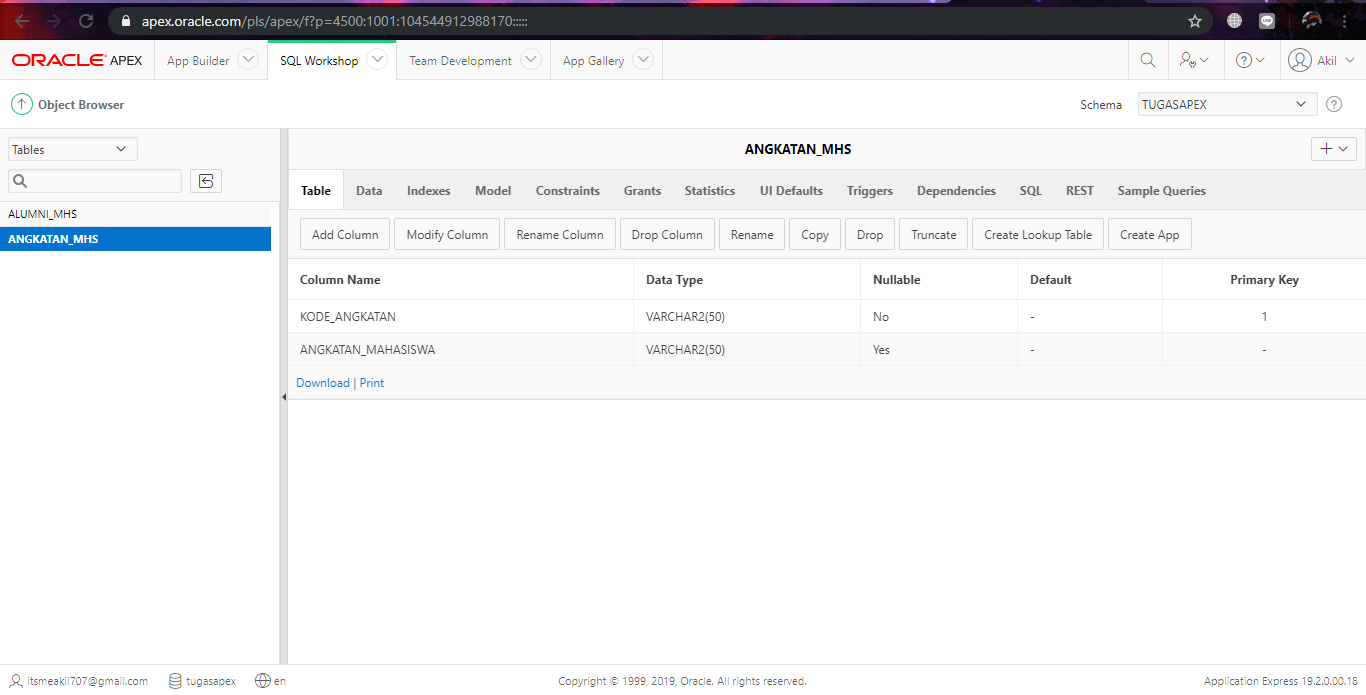
\includegraphics[width=.8\textwidth]{figure/30.PNG}
    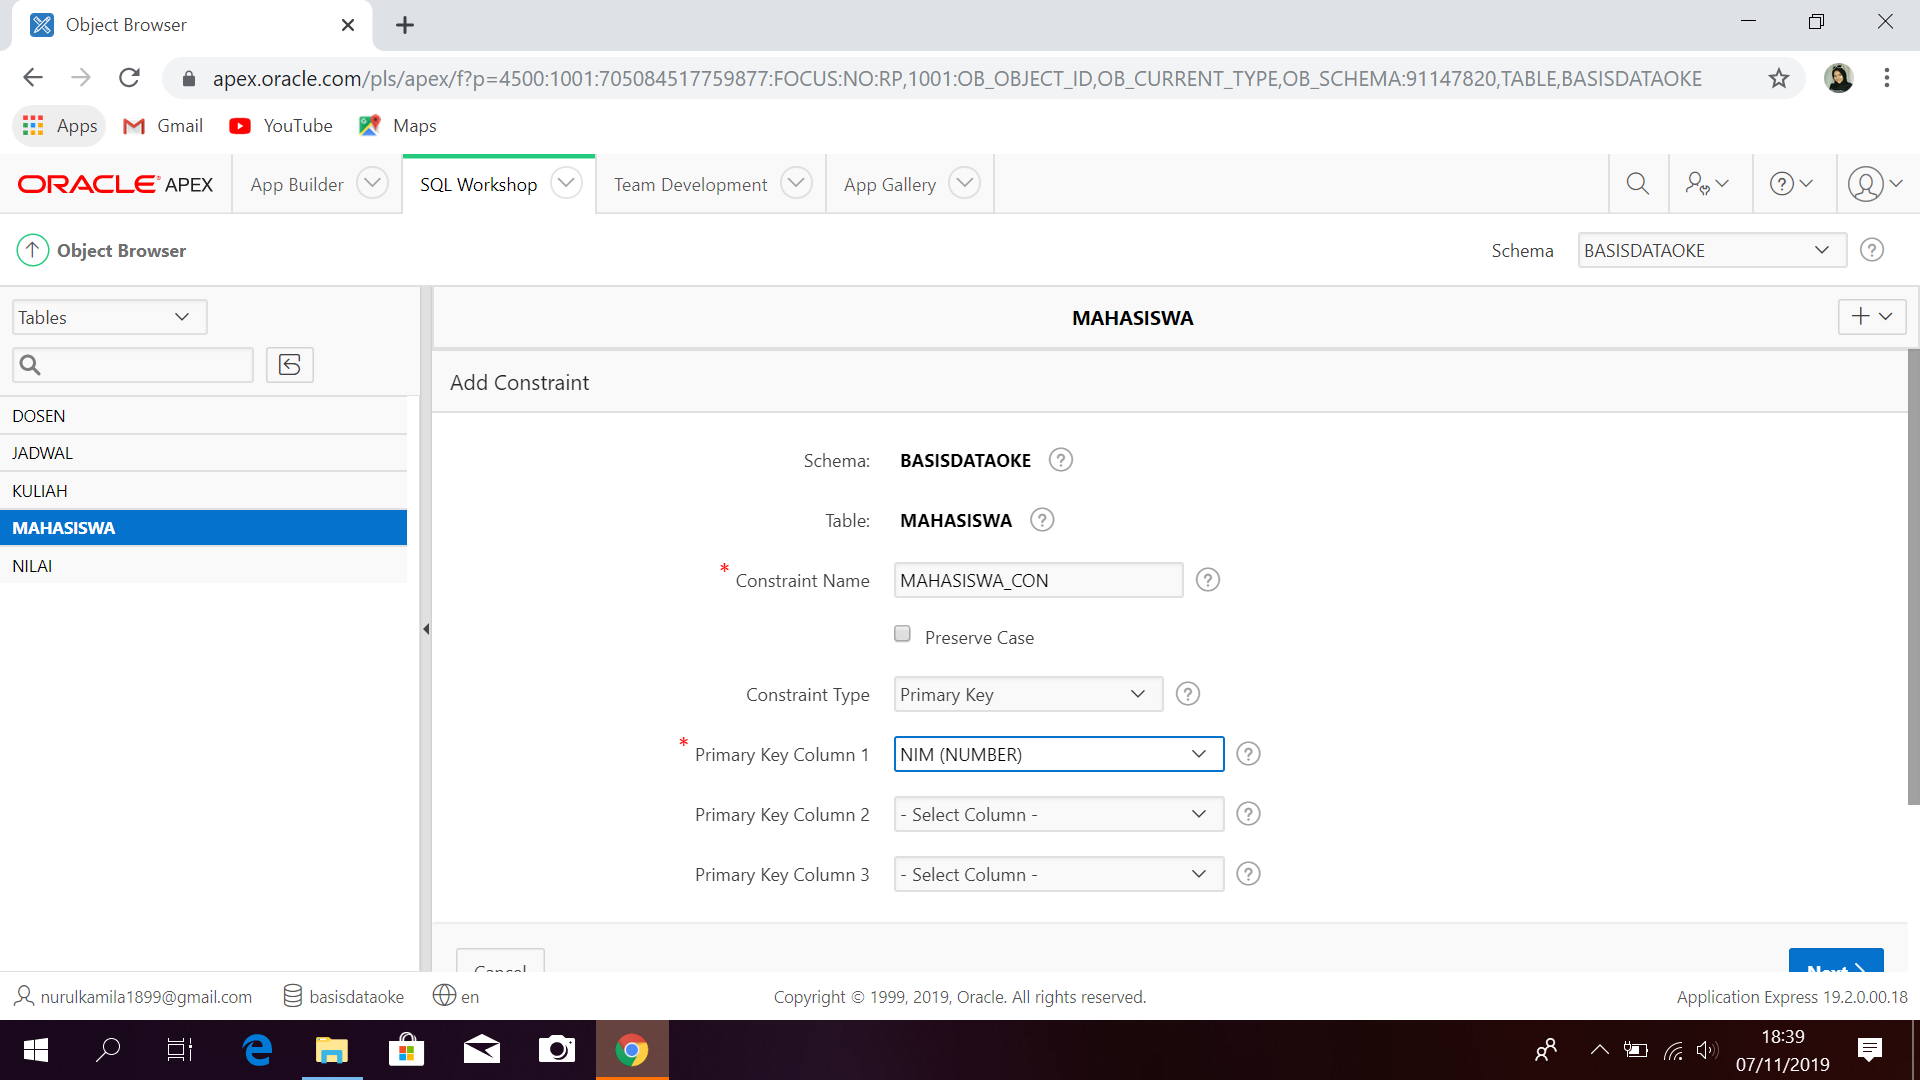
\includegraphics[width=.8\textwidth]{figure/31.PNG}
    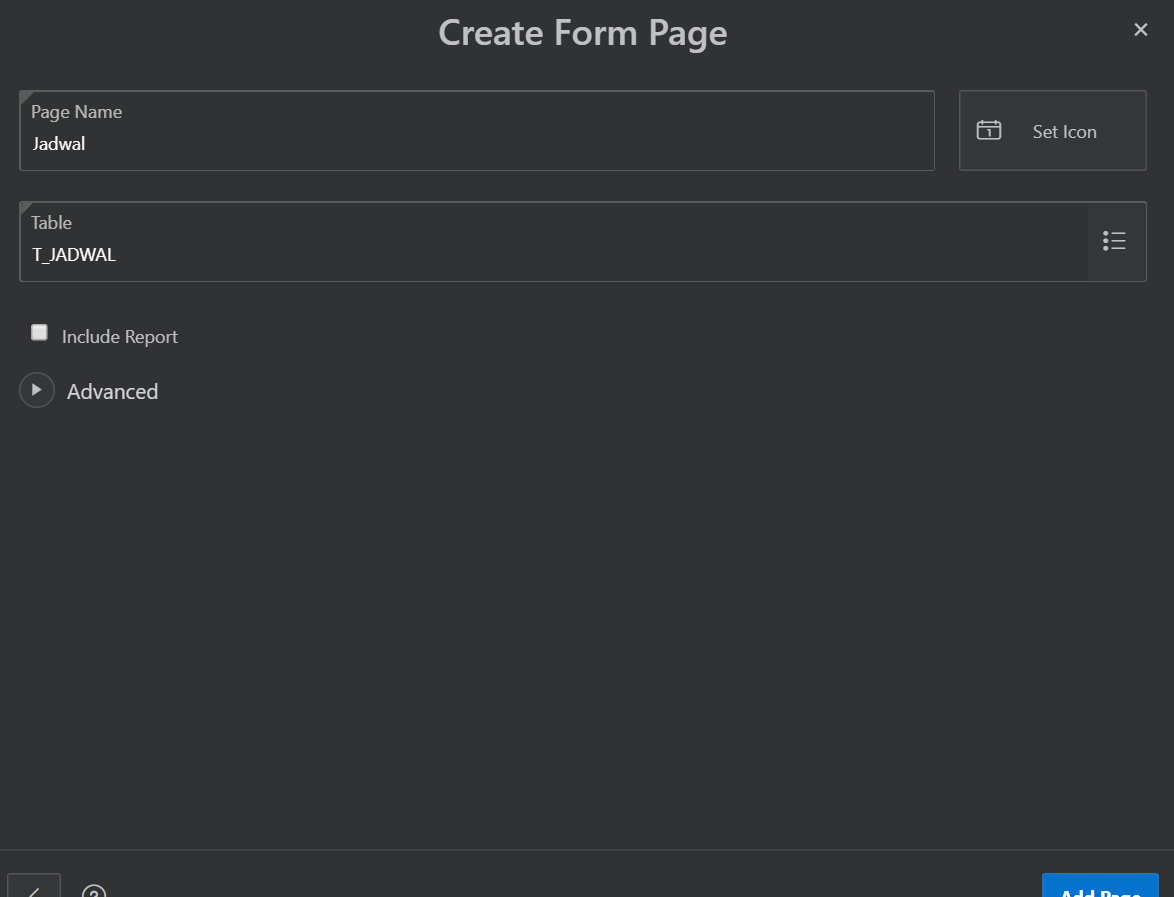
\includegraphics[width=.8\textwidth]{figure/32.PNG}
    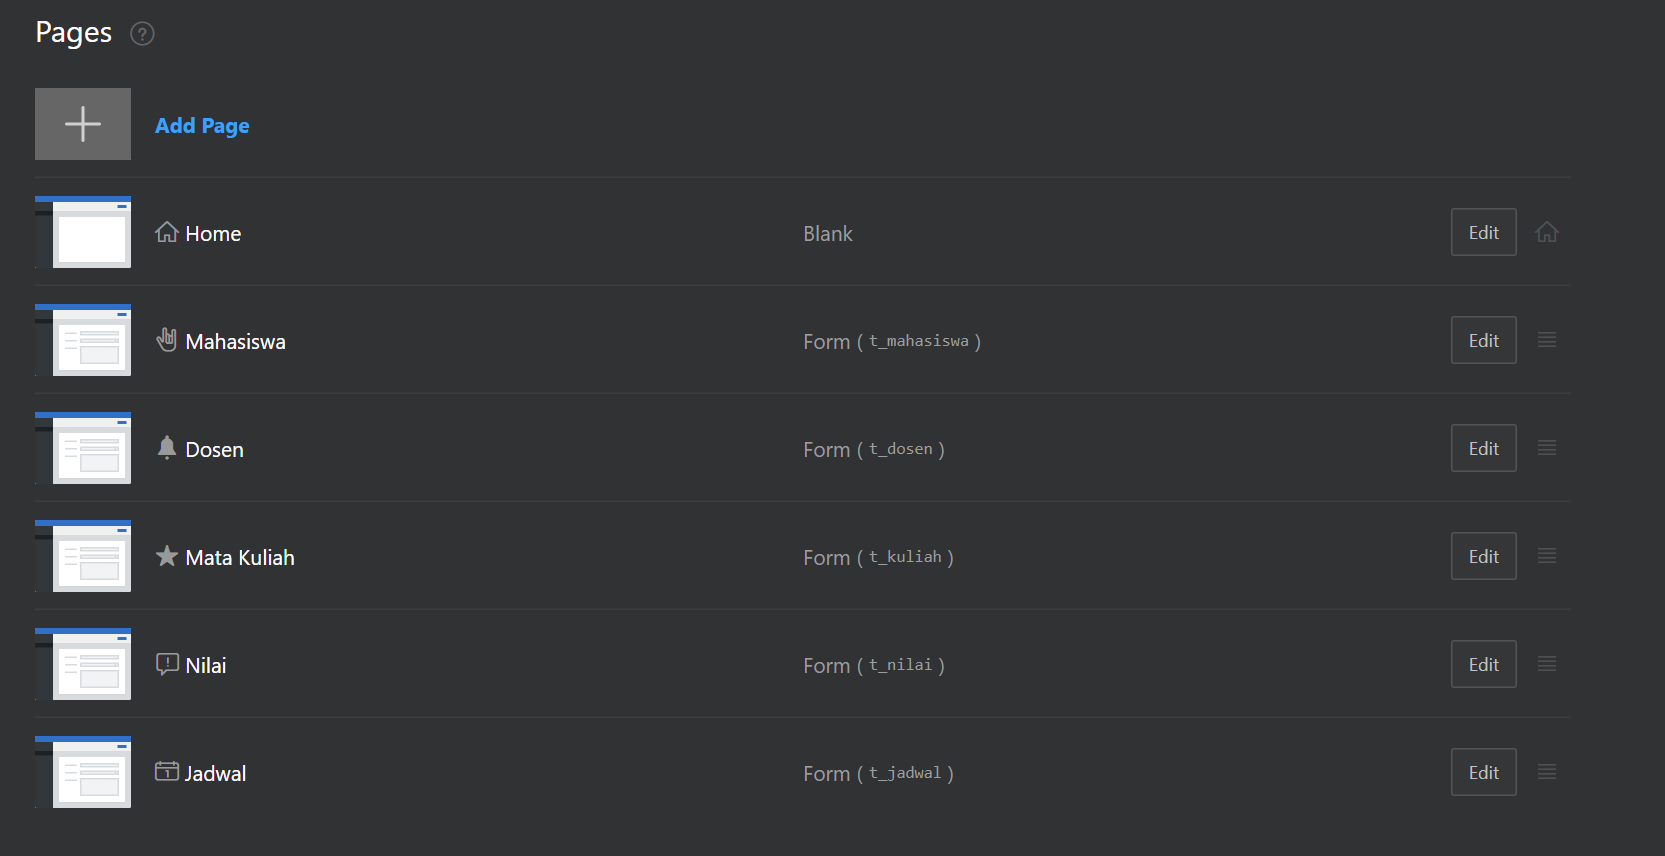
\includegraphics[width=.8\textwidth]{figure/33.PNG}
    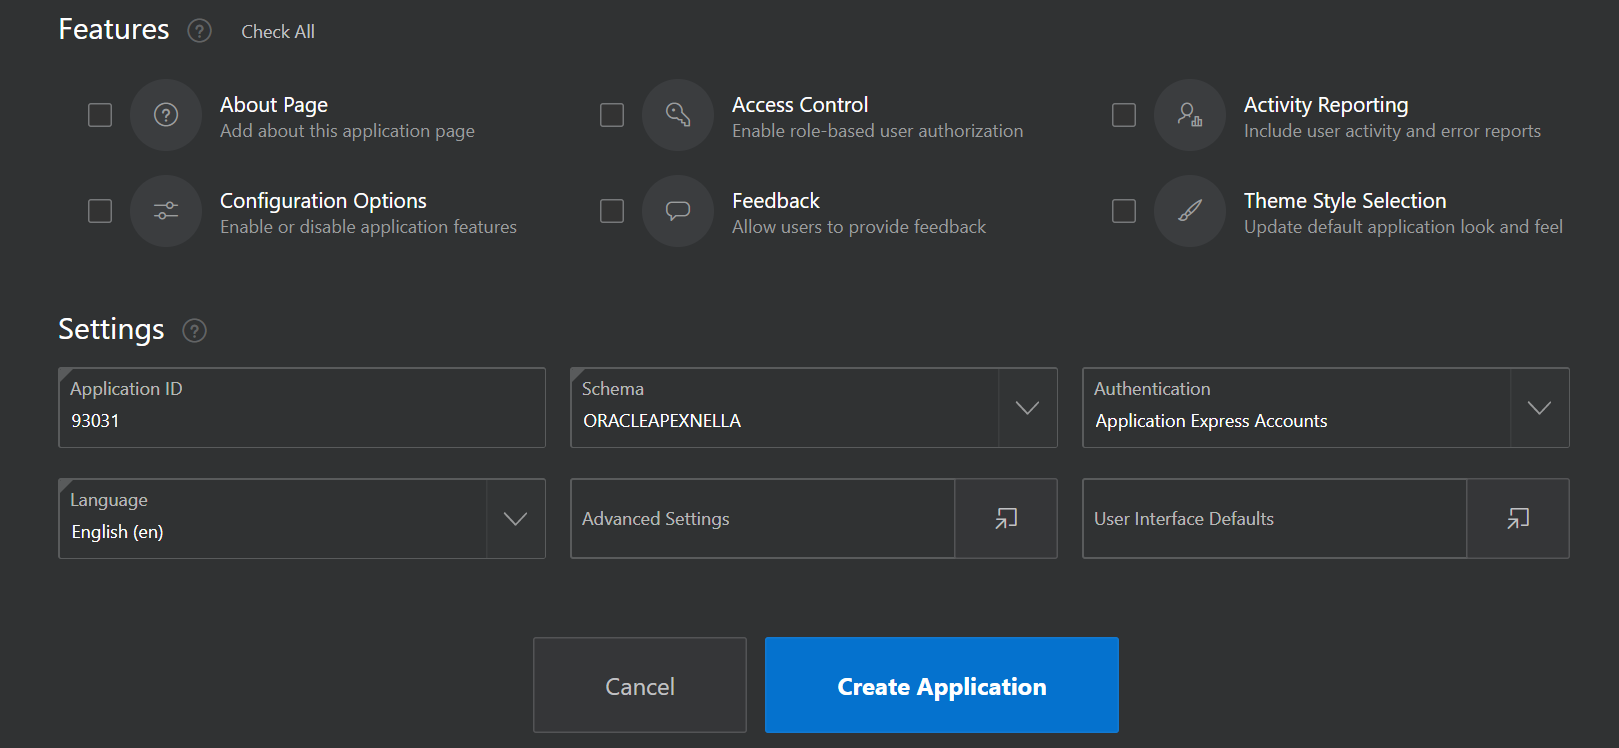
\includegraphics[width=.8\textwidth]{figure/34.PNG}
    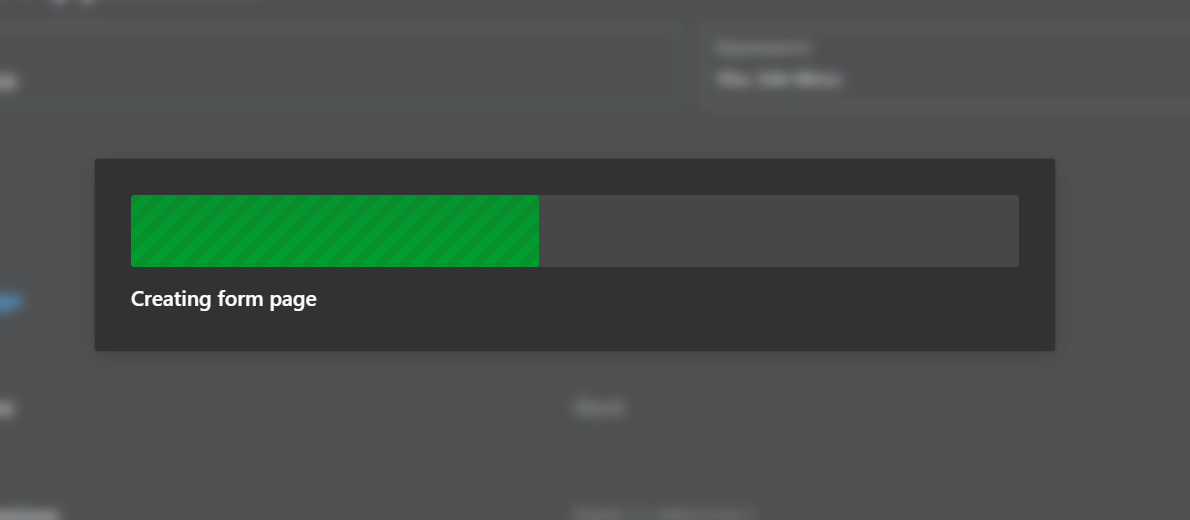
\includegraphics[width=.8\textwidth]{figure/35.PNG}
    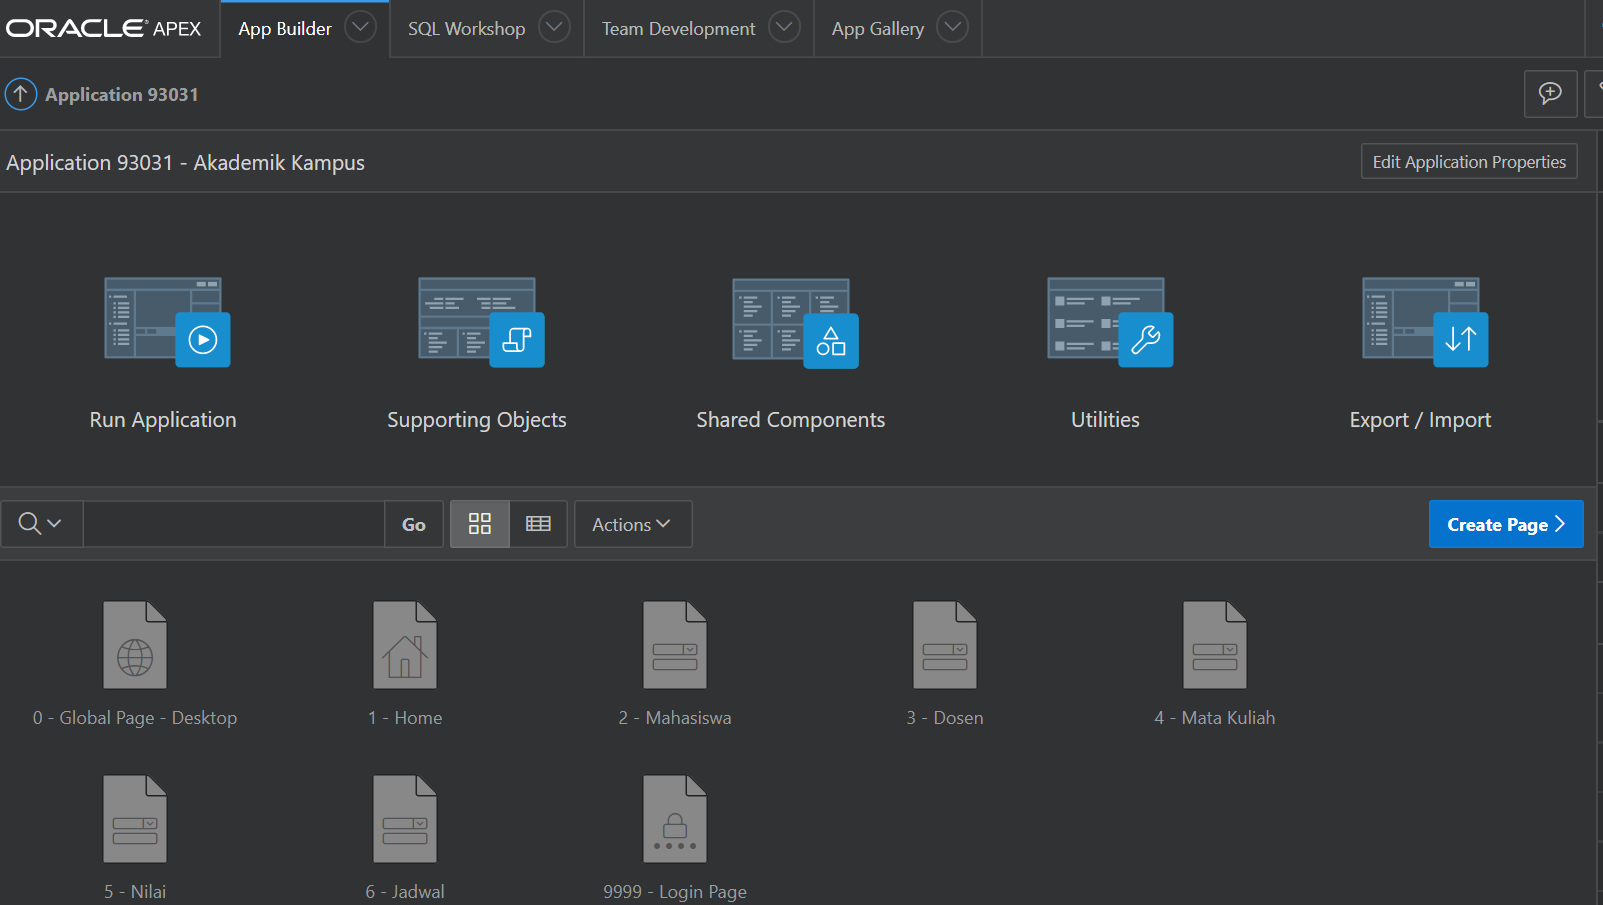
\includegraphics[width=.8\textwidth]{figure/36.PNG}
    \end{center}
    \item Lalu, kembali ke App Builder, lalu pilih New Application
     \begin{center}
    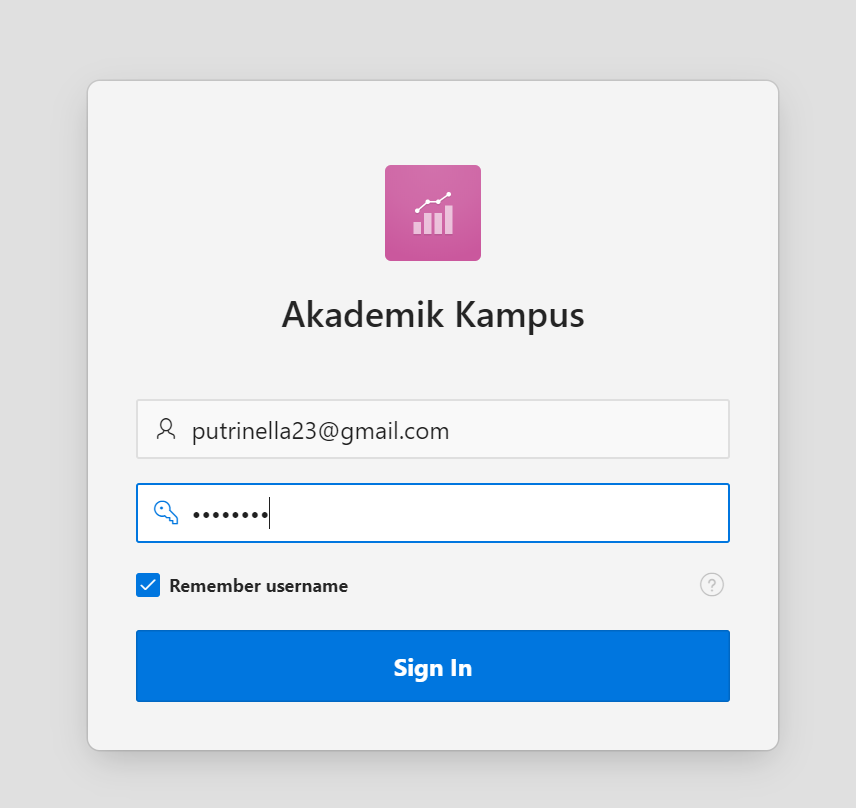
\includegraphics[width=.8\textwidth]{figure/37.PNG}
    \end{center}
    \item Add Page , lalu pilih Interactive Report atau add page yang lain.
     \begin{center}
    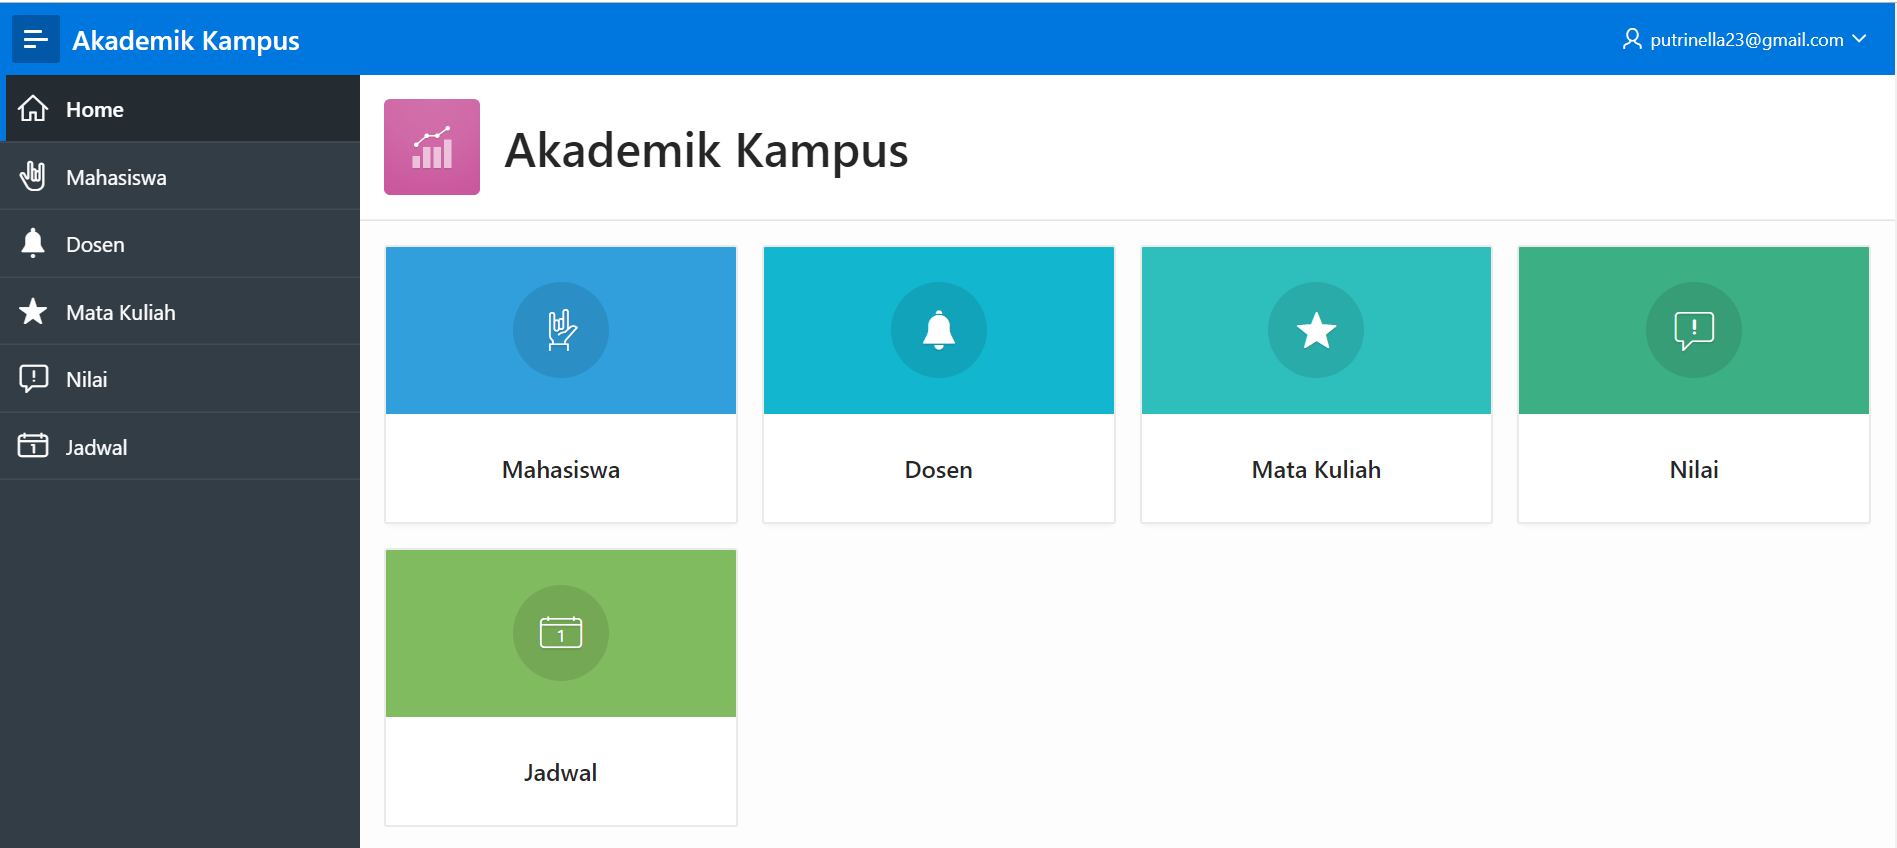
\includegraphics[width=.8\textwidth]{figure/38.PNG}
     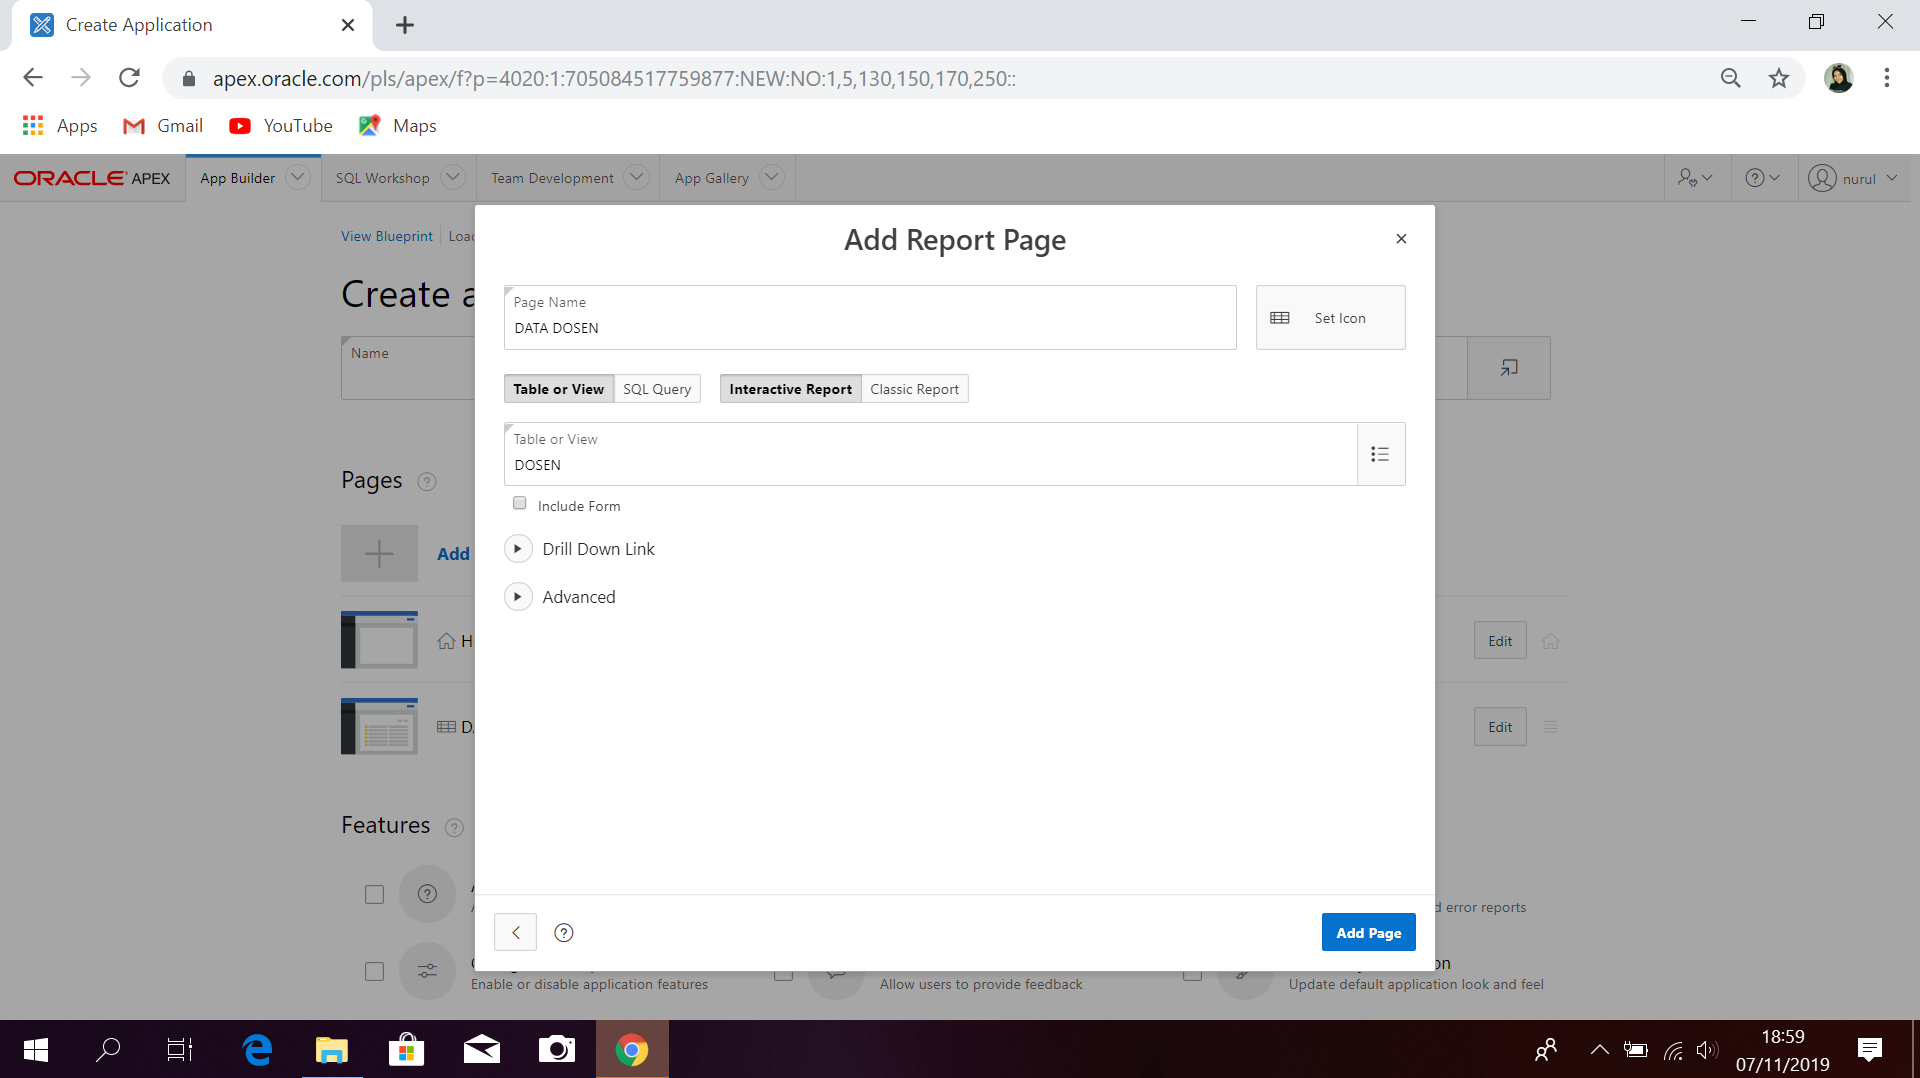
\includegraphics[width=.8\textwidth]{figure/39.PNG}
      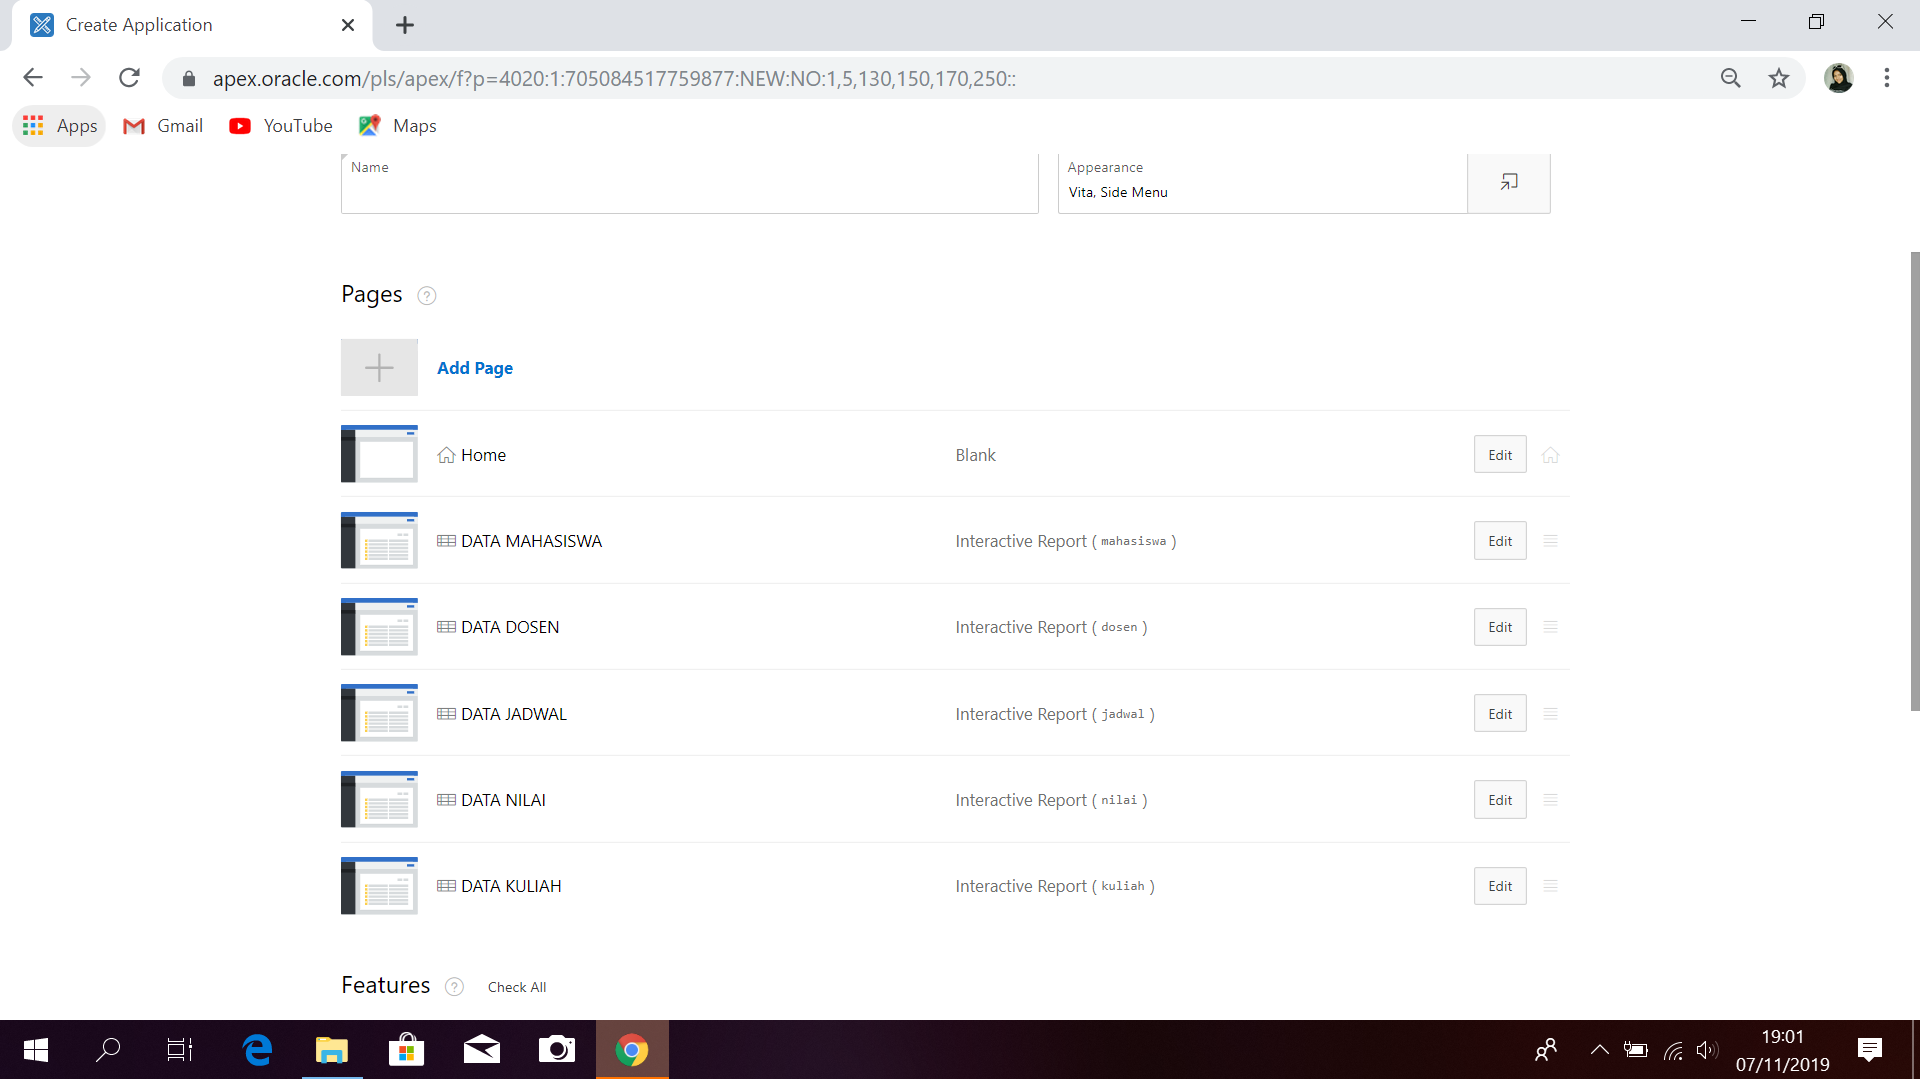
\includegraphics[width=.8\textwidth]{figure/40.PNG}
       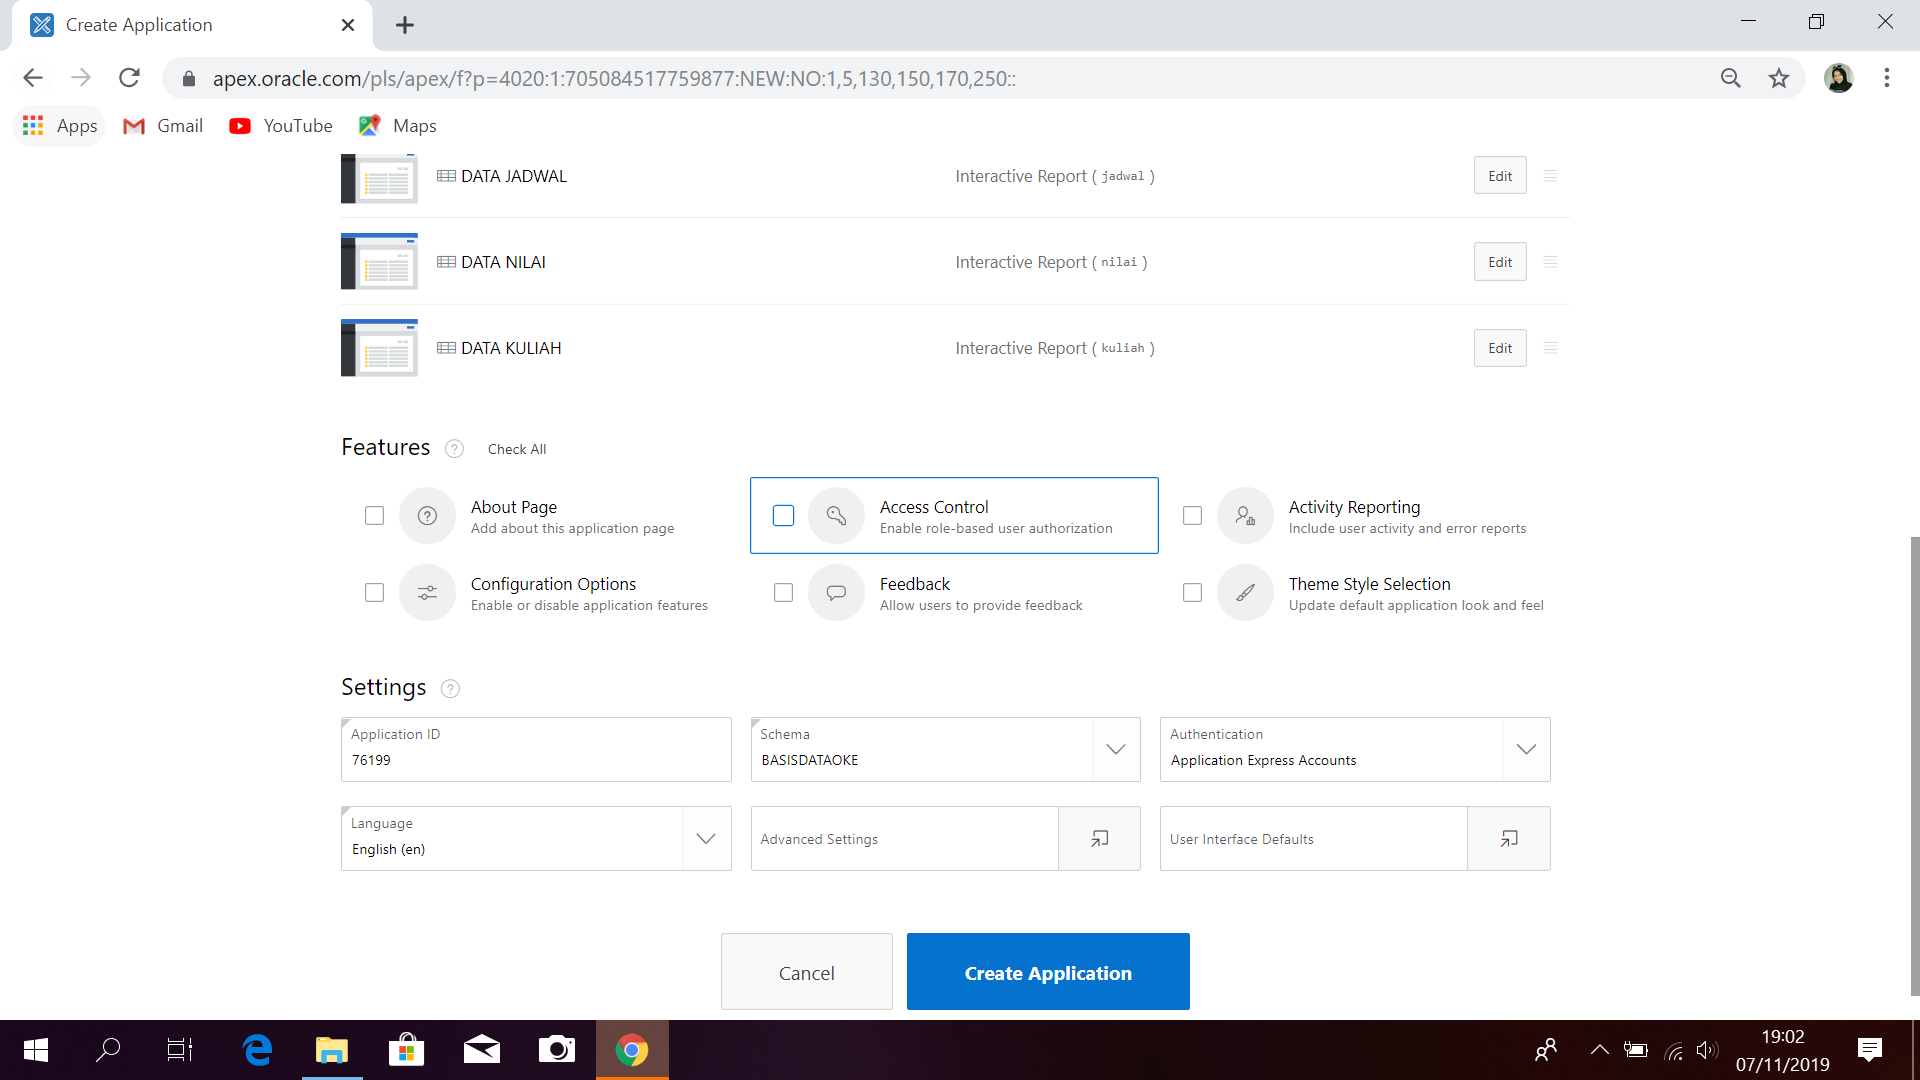
\includegraphics[width=.8\textwidth]{figure/41.PNG}
    \end{center}
    \item jika sudah semua, Run Application. Aplikasi sudah siap dibuka.
     \begin{center}
    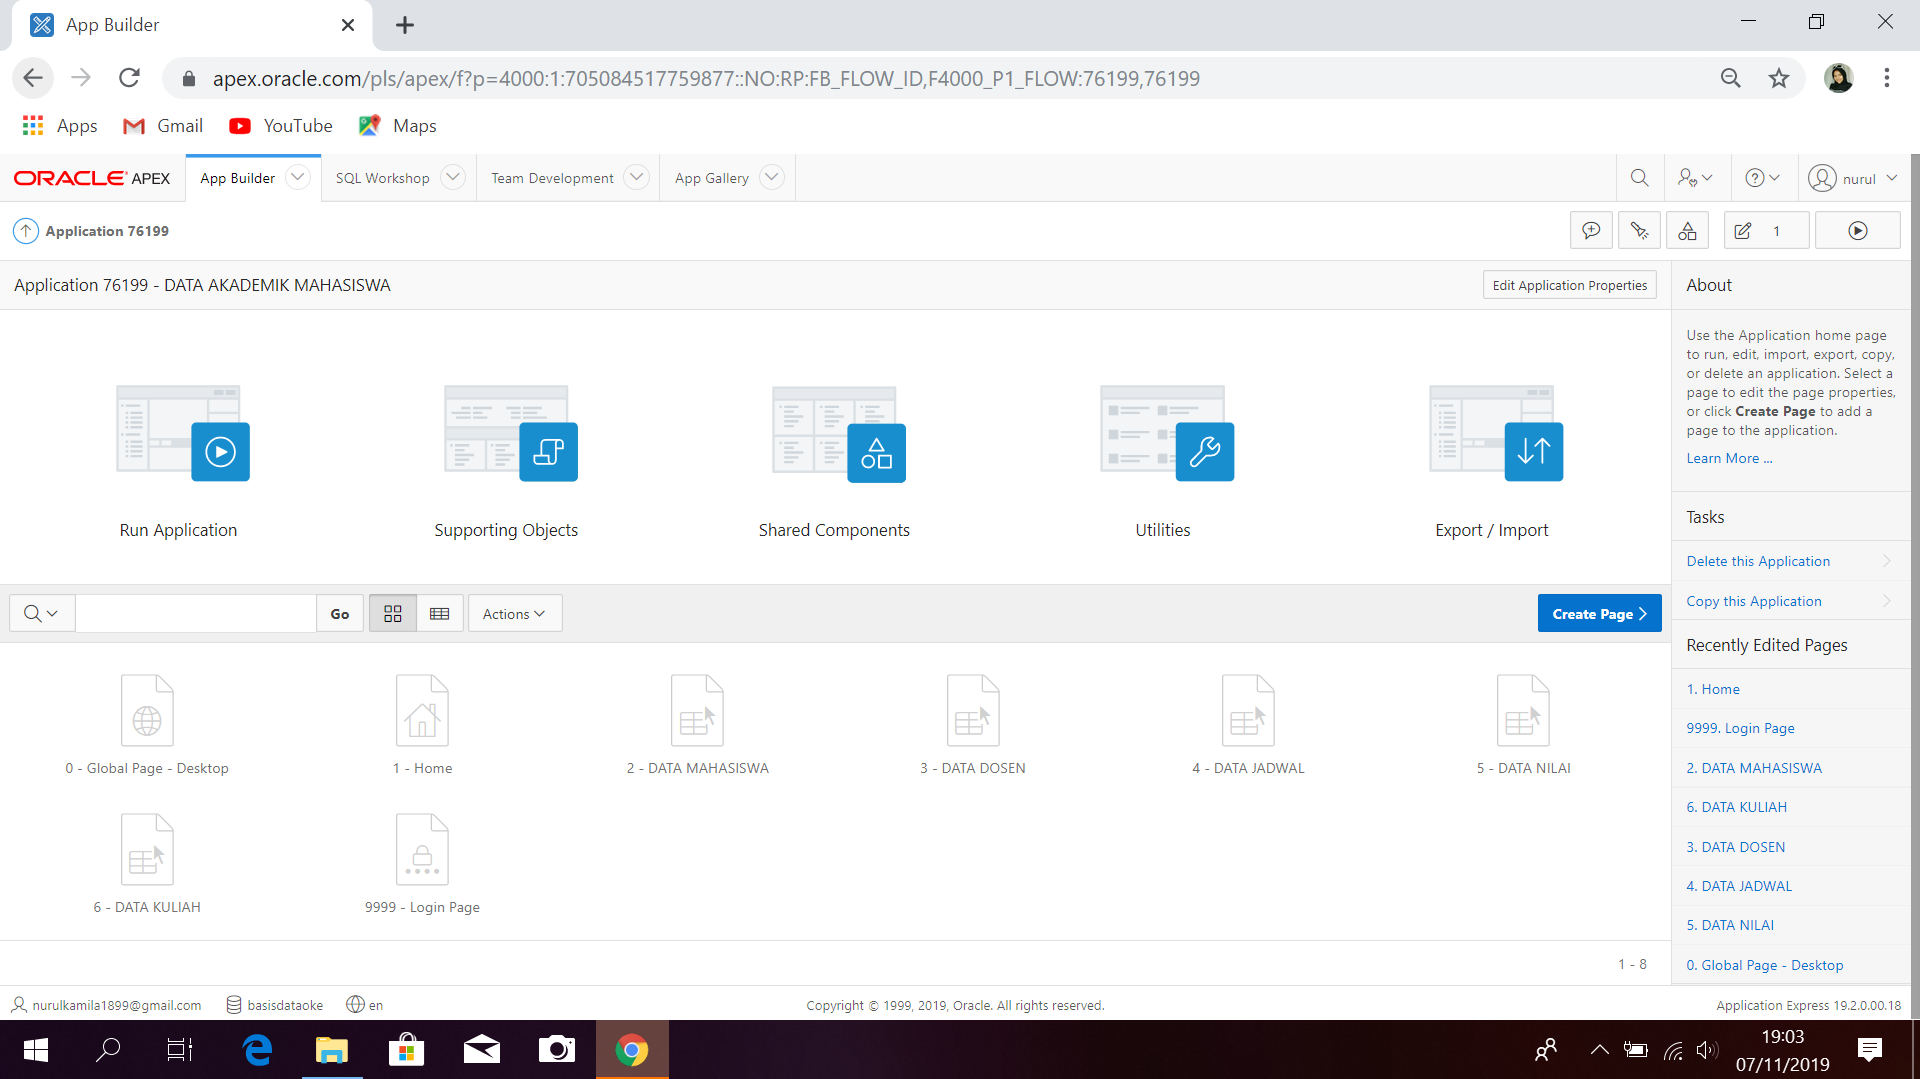
\includegraphics[width=.8\textwidth]{figure/42.PNG}
    \includegraphics[width=.8\textwidth]{figure/akhir.png}
    \includegraphics[width=.8\textwidth]{figure/akhir2.png}
    \end{center}
\end{enumerate}

\section{link login  
https://apex.oracle.com/pls/apex/f?p=92605:LOGIN_DESKTOP:5784700124136:::::\\
Username : murnialestari2@gmail.com\\
Password :murnia123}


\end{document}
